\documentclass{uflamon}          % classe base para a monografia

%==============================================================================
% Utilizacao de pacotes
\usepackage[T1]{fontenc}         % usa fontes postscript com acentos
\usepackage[brazil]{babel}       % hifenização e títulos em português do Brasil
\usepackage[utf8]{inputenc}     % permite edição direta com acentos
\usepackage{amsmath}             % pacote da AMS para Matemática Avançada
\usepackage{amssymb}             % símbolos extras da AMS
\usepackage{latexsym}            % símbolos extras do LaTeX
\usepackage{graphicx}            % para inserção de gráficos
\usepackage{listings}            % para inserção de código
\usepackage{fancyvrb}            % para inserção de saídas de comandos
%\usepackage{enumerate}           % para personalizar lista enumeradas 
											%(incluso na classe)
\usepackage{longtable}           % para tambelas muito grandes NOVO!!!!

\usepackage{colortbl} % cores em tabelas
\newcolumntype{Z}{|>{\columncolor[gray]{0.9}}l|} %cor cinza em células
%\usepackage{array} % já incluso na classe
\newcolumntype{L}[1]{>{\raggedright\let\newline\\\arraybackslash\hspace{0pt}}m{#1}}
\newcolumntype{C}[1]{>{\centering\let\newline\\\arraybackslash\hspace{0pt}}m{#1}}
\newcolumntype{R}[1]{>{\raggedleft\let\newline\\\arraybackslash\hspace{0pt}}m{#1}}
\usepackage{multirow} % para juntar duas linhas em uma só

\usepackage{multicol} % para uso de várias colunas

% cores para os links cruzados
\usepackage{color}
\definecolor{rltred}{rgb}{0.2,0,0}
\definecolor{rltgreen}{rgb}{0,0.2,0}
\definecolor{rltblue}{rgb}{0,0,0.2}

\usepackage[colorlinks=true,
            urlcolor=rltblue,       % \href{...}{...} external (URL)
            filecolor=rltgreen,     % \href{...} local file
            linkcolor=rltred,       % \ref{...} and \pageref{...}
            citecolor=rltgreen,
            pdftitle={TccLuizVersaoFinal},
          pdfauthor={Luiz Otávio Andrade Soares},
          pdfsubject={Comparação do desempenho de Java, Go HTTP e gRPC em aplicações distribuídas},
          pdfkeywords={Comunicação Científica. 2. Pesquisa . 3. Pesquisa Científica. 
 					 4. Redação. 5. Monografia.}%
]{hyperref} % para referência cruzadas
%\usepackage{hyperref}            % para referência cruzadas
\usepackage{subfigure}           % figuras dentro de figuras
\usepackage{caption}            % remodelando o formato dos títulos de 
                                 % tabelas e figuras

% configuração padrão do listings   
\lstset{
   language=Java,
   extendedchars=true,
   tabsize=3,
   basicstyle=\footnotesize\ttfamily,
   stringstyle=\em,
   showstringspaces=false 
}

% para referências de acordo com a ABNT
% precisa instalar o abntex2 antes!!!
% http://abntex.codigolivre.org.br/
% comente se pretende usar outro padrão

%abnt-emphasize=bf coloca o título das bibliografias em negrito
%abnt-thesis-year=both
\usepackage[alf,abnt-etal-cite=3,abnt-etal-list=3,abnt-url-package=url,abnt-emphasize=bf]{abntex2cite}
\usepackage{colortbl}

% evite usar o hyperref com abntex, pode dar caca em urls... no linha anterior, informo
% para incluir urls usando o pacote url e não o hyperref
%
% caso queira o hyperref com abntex, comente a linha anterior e descomente a seguinte
%\usepackage[alf,abnt-etal-cite=3,abnt-etal-list=0,abnt-etal-text=emph]{abntex2cite}
%
% caso vc ainda use a versão anterior da abntex, comente a linha incluindo o abntex2cite
% e descomente a próxima linha 
%\usepackage[alf,abnt-etal-cite=3,abnt-etal-list=0,abnt-etal-text=emph]{abntcite}


% redefinindo formatação de títulos de tabelas e figuras


%==============================================================================
% para os fãs do Word, descomente as linhas abaixo
%\sloppy %mais espaço entre as linhas
%\usepackage{identfirst} %identando-se a primeira linha de cada seção
%\noindentfirst % Tire o comentário para manter o padrão do LaTeX.

%============================================================================
% definido comandos na monografia - não é necessário na sua monografia 
% apenas para exemplificar a definição de novos comandos
\newcommand{\defs}[1]{\textsl{#1}}
\newcommand{\mcode}[1]{$\mathtt{#1}$}
\newcommand{\pargenerico}[2]{\mcode{({#1},{#2})}}
\newcommand{\gogrpc}{\pargenerico{Go}{gRPC}}
\newcommand{\gorest}{\pargenerico{Go}{REST}}
\newcommand{\javagrpc}{\pargenerico{Java}{gRPC}}
\newcommand{\javarest}{\pargenerico{Java}{REST}}

\newcommand{\okterra}[1]{\textcolor{blue}{#1}}
\newcommand{\okterrasblp}[1]{\textcolor{black}{#1}}
\newcommand{\noterrasblp}[1]{}
\newcommand{\aspas}[1]{{``#1''}}
\newcommand{\aspassimples}[1]{{`#1'}}



% Especificando hifenizações que por ventura LaTeX não saiba fazer
% Por padrão 99,9% dos termos em português devem ser hifenizados corretamente.
\hyphenation{hardware software Li-nux am-bien-te diag-nos-ti-car coor-de-na-ção 
FAE-PE Recovery TelEduc Williams UFLA}

%==============================================================================
% Dados da monografia, capa: autor, titulo, banca, etc... - SUBSTITUA DE ACORDO
%==============================================================================
\author{Luiz Otávio Andrade Soares}
\title{Go x Java e gRPC x REST: Um estudo empírico}
\engtitle{Go vs. Java and gRPC vs. REST: An Empirical Study}
\date{2024}
\tipo{Artigo apresentado à Universidade Federal de Lavras, como parte das exigências do Curso de Ciência da Computação, para a obtenção do título de Bacharel.}
% use \orientador ou \orientadora quando for o caso
\orientador{Prof. DSc. Ricardo Terra Nunes Bueno Vilela}
%\orientadora{}
% use \coorientador ou \coorientadora quando for o caso
% \coorientador{Prof. DSc. Rafael Serapilha Durelli} % comente se não tiver coorientador
%\coorientadora{}
\local{Lavras -- MG}
\bancaum{Prof. DSc. Ricardo Terra Nunes Bueno Vilela}{DCC - UFLA}
\bancadois{Prof. DSc. Rafael Serapilha Durelli}{DCC - UFLA} % comente se sua banca tiver só um professor
\bancatres{Prof. DSc. Mayron César de Oliveira Moreira}{DCC - UFLA}
\defesa{19 de Julho de 2024}
%==============================================================================
%##################################################
% Dados para Ficha catalográfica, gerada pelo sistema da Biblioteca da UFLA
% http://www.biblioteca.ufla.br/FichaCatalografica/
% dados para ficha catalográfica
% Elaboração da Ficha Catalográfica
\preparofichacat{Ficha catalográfica elaborada pela Coordenadoria de Processos Técnicos \\ da Biblioteca Universitária da UFLA}
% primeiro autor - como na primeira linha da ficha catalográfica
\fcautor{Soares, Luiz Otávio Andrade}
% autores, separados por vírgula - na ficha catalográfica, no formato que
% vem após o título e a barra ("/")
\fcautores{Luiz Otávio Andrade Soares}
% caso trabalho seja ilustrado (figuras, gráficos, tabelas, etc.), 
% então informar por meio do comando a seguir
% caso não seja ilustrado, basta comentá-lo
% \fcilustrado{il.}
% dados da edição para a ficha 
\fcedicao{2$^a$ ed. rev., atual. e ampl.}
% tipo do trabalho (tese, dissertação, etc.), de acordo com sistema
% de geração de ficha catalográfica
\fctipo{Monografia(graduação)}
% ano da defesa, só precisa informar se for diferente do ano da publicação
% se forem iguais, comente a linha a seguir
\fcdatadefesa{2024}
% preencher aqui com os dados de catalogação gerados pelo sistema
\fccatalogacao{1. TCC. 2. Monografia. 3. Dissertação. 4. Tese. 5. Trabalho Científico – Normas. I. Universidade Federal de Lavras. II. Título.}
\fcclasi{808.066}

%##################################################

%\antesfichacat{\noindent Para citar este documento: \\UNIVERSIDADE FEDERAL DE LAVRAS. Biblioteca Universitária. \textbf{Manual de normalização e estrutura de trabalhos acadêmicos: TCC, monografias, dissertações e teses}. 2. ed. rev., atual. e ampl. Lavras, 2015. Disponível em: \url{http://www.biblioteca.ufla.br/wordpress/wpcontent/uploads/bdtd/manual_normalizacao_UFLA.pdf}. Acesso em: data de acesso.}

%\depoisfichacat{\noindent A reprodução e a divulgação total ou parcial deste trabalho são autorizadas, por qualquer meio convencional ou eletrônico, para fins de estudo e pesquisa, desde que citada a fonte.\\
%\newline
%{\small Este documento possui páginas em branco para facilitar a impressão frente-e-verso.}}

%##################################################

%##################################################

% para os exemplos do manual
%\newenvironment{exemplomanual}{
%\vspace{0.5cm}
%\noindent\begin{minipage}{\textwidth}
%\noindent\rule{\textwidth}{0.5pt}
%\vspace{-1cm}
%\begin{flushleft}
%}{
%\end{flushleft}
%\vspace{-0.6cm}
%\noindent\rule{\textwidth}{0.5pt}
%\vspace{0.3cm}
%\end{minipage}
%}

%\newenvironment{exemplomanuallista}{
%\vspace{0.3cm}
%\noindent\begin{minipage}{\textwidth - 0.5cm}
%\noindent\rule{\textwidth}{0.5pt}
%\vspace{-1cm}
%\begin{flushleft}
%}{
%\end{flushleft}
%\vspace{-0.6cm}
%\noindent\rule{\textwidth}{0.5pt}
%\vspace{0.3cm}
%\end{minipage}
%}

% por conta de alguns exemplos
%\usepackage{setspace}

%##################################################

% se vc já defendeu e tem o arquivo escaneado da folha de rosto, 
% descomente e altere o nome do arquivo
%\folhaAprovacaoAssinada{folharosto}

% Aqui começa o documento propriamente dito
\begin{document}

\maketitle

\dedic{À minha família, amigos e ao meu amor}     % Dedicatórias\\

\thanks{
Primeiramente, agradeço à minha família, cujo apoio incondicional foi fundamental durante toda esta jornada.
Um agradecimento especial à minha avó Maria Alice, que não apenas me inspirou com sua sabedoria e carinho, mas também viabilizou a minha oportunidade de estudar fora.
Sem o seu apoio, essa conquista não seria possível.
Sua generosidade e dedicação são fontes de força e motivação que levarei comigo para sempre.

À minha mãe Eva, que sempre acreditou no meu potencial e me incentivou a seguir em frente, mesmo nos momentos mais desafiadores, meu profundo agradecimento.
Ao meu irmão João Bruno, que, com sua amizade e carinho, tornou cada etapa deste caminho mais leve e significativa.

Gostaria de agradecer também à minha república, Último Gole, por todos os momentos de descontração e companheirismo, que foram essenciais para manter o equilíbrio durante os estudos.
A convivência com vocês foi uma parte importante da minha experiência universitária, e sou grato por cada instante compartilhado.

Um agradecimento especial à minha namorada, Laura Sarto, pelo apoio, paciência e por estar ao meu lado em todos os momentos, celebrando as conquistas e oferecendo conforto nas dificuldades.
Sua presença foi um alicerce sólido ao longo desta jornada.

Por fim, agradeço a todos que, de alguma forma, contribuíram para a realização deste trabalho.
Agradeço a todos os professores, amigos e colegas que fizeram parte dessa trajetória.
}         % Agradecimentos

\epigrafe{ % citação opcional
No meio do caminho tinha uma pedra, tinha uma pedra no meio do caminho.\\
(Carlos Drummond de Andrade)}

% palavras-chave
\palchaves{Linguagens de programação, estilo arquitetural de comunicação, estudo empírico}

\resumo{Este trabalho investiga a influência das linguagens de programação Java e Go e das arquiteturas de comunicação REST e gRPC no desempenho de APIs. A questão de pesquisa~\#1 investigou qual par {\em (linguagem,arquitetura-comunicação)} provê melhor desempenho. Por um lado, pares \gogrpc{} e \javagrpc{} se destacaram em requisições de tamanhos usuais ({\em StdSize}) possivelmente devido à eficiência na compactação de dados e na redução de latência oferecida pelo gRPC. Por outro lado, pares \gorest{} e \javarest{} se destacaram em requisições de grande volume~({\em LargeSize}) provavelmente devido à flexibilidade do REST em lidar com grandes volumes de dados sem estrutura rígida. A questão de pesquisa \#2, de forma complementar, investigou a influência de cada fator no desempenho. Um projeto fatorial $2^kr$ concluiu que enquanto a linguagem de programação exerce uma influência de 2\%, a arquitetura de comunicação influencia 94\%.}  % Resumo (digite aqui o resumo)

% keywords devem vir antes do abstract
\keywords{Programming Languages, Communication Architectural Style, Empirical Study} % keywords
\abstract{This study investigates the influence of the Java and Go programming languages and the REST and gRPC communication architectures on the performance of APIs. Research Question \#1 examined which pair (language, communication architecture) provides better performance. On one hand, the pairs (Go, gRPC) and (Java, gRPC) excelled in standard-size requests (StdSize), possibly due to the efficiency in data compression and latency reduction offered by gRPC. On the other hand, the pairs (Go, REST) and (Java, REST) stood out in handling large-volume requests (LargeSize), likely due to REST's flexibility in managing large data volumes without a rigid structure. Complementarily, Research Question \#2 investigated the influence of each factor on performance. A 2kr factorial design concluded that while the programming language exerts a 2\% influence, the communication architecture influences 94\%.}

%##################################################

% Dados do guia
%\begin{titlepage}
%\pagestyle{empty}
%\renewcommand{\baselinestretch}{1}
%\enlargethispage{1.5cm}
%\input{reitoria}
%\cleardoublepage
%\end{titlepage}

%##################################################

% descomente para habilitar a lista desejada
\listoffigures                             % Lista de Figuras
%\listofilustracoes
%\listofgraficos							   % Lista de Gráficos
\listoftables                              % Lista de Tabelas
% \listofquadros							   % Lista de Quadros
%\listofexemplos
%\listofteoremas
\tableofcontents                           % Sumário

\clearpage

\pagestyle{ufla}

%==============================================================================
% incluindo os capitulos
\chapter{INTRODUÇÃO}

As APIs ({\em Application Programming Interfaces}) desempenham um papel crucial no desenvolvimento de sistemas,
facilitando a integração e comunicação entre diferentes sistemas de software e plataformas, 
permitindo assim uma maior modularidade, escalabilidade e reutilização de código~\cite{apiArchitecture}.
%
Na prática usual adotada por fábricas de software, utiliza-se o protocolo HTTPS~(\textit{Hypertext Transfer Protocol Secure}) para 
facilitar a comunicação e transferência de dados na Internet
e o estilo arquitetural de comunicação REST (\textit{Representational State Transfer}) 
para organizar e acessar serviços web de maneira padronizada~\cite{rfc2616, fielding2000architectural}.
Isso se consolidou como o padrão usual para a criação de sistemas distribuídos robustos~\cite{restPop, apiArchitecture, restRefact}.

A ascensão de Go e gRPC, promovida significativamente pelo Google, marca uma evolução nas tecnologias de desenvolvimento de software~\cite{go2012, grpc2015}. Go destaca-se pela sua simplicidade e eficiência no manejo de operações concorrentes, enquanto gRPC revitaliza o conceito de chamadas de procedimento remoto (RPC) ao integrar funcionalidades do HTTP/2, facilitando comunicações rápidas e eficientes por meio de \textit{Protocol Buffers} para serialização de dados. Essas características são particularmente benéficas para microsserviços e aplicações que demandam alto desempenho e baixa latência.

\noterrasblp{
Na literatura atual, é comum encontrar estudos comparativos de tecnologias que frequentemente apresentam metodologias pouco definidas \cite{javaVsGo, kaminski2023comparative,optimalPythonR}. 
Além disso, nota-se a falta de rigor na aplicação de métodos estatísticos para a análise dos resultados, ou até ausência de métodos estatísticos \cite{restGraphqlGrpc,kaminski2023comparative, berg2023benchmarking}. A maioria desses estudos se baseia em experimentos práticos sem uma estrutura metodológica robusta, o que pode limitar a validade e a confiabilidade das conclusões. Em contraste, este trabalho se diferencia ao empregar uma metodologia bem definida e o uso de métodos estatísticos rigorosos para corroborar as análises.
}

Este artigo, portanto, conduz um estudo empírico que emprega procedimentos estatísticos rigorosos para quantificar as melhorias oferecidas por uma linguagem de programação e um estilo arquitetural de comunicação considerados promissores.
%
Partindo da presunção de que Java é uma linguagem consolidada no mercado, assim como REST é quase sempre adotado
como o estilo arquitetural de comunicação, este estudo 
(i)~investiga a combinação mais eficiente entre as linguagens de programação Go e Java e os estilos arquiteturais de
comunicação gRPC e REST e
(ii)~quantifica a influência da linguagem de programação e do estilo arquitetural de comunicação na eficiência.

A partir de quatro implementações -- \gogrpc{}, \gorest{}, \javagrpc{} e \javarest{} -- de uma
mesma aplicação, a questão de pesquisa \#1 investigou qual par {\em (linguagem,arquitetura-comunicação)} provê melhor desempenho e comprovou diferença estatística entre todos os pares. Além disso, as análises indicaram que os pares \gogrpc{} e \javagrpc{} se destacam em requisições de tamanhos usuais~({\em StdSize}) 
possivelmente devido à eficiência na compactação de dados e na redução de latência oferecida pelo gRPC.
Por outro lado, pares \gorest{} e \javarest{} se destacaram em requisições de grande volume~({\em LargeSize})
provavelmente devido à flexibilidade do REST em lidar com grandes volumes de dados sem estrutura rígida.
%
A questão de pesquisa \#2, de forma complementar, investigou a influência de cada fator no desempenho por meio de um projeto fatorial $2^kr$. Essa análise concluiu que a linguagem de programação exerce uma influência de 2\%, enquanto que
a arquitetura de comunicação influencia 94\%.   

Este documento está organizado como a seguir. A Seção~\ref{sec:artigo} contém o artigo completo, enquanto a seção~\ref{cap:conclusao} contém considerações finais acerca do estudo conduzido.

% \chapter{REFERENCIAL TEÓRICO}

\subsection{Kubernetes}

A programação paralela e distribuída é uma área de pesquisa que se concentra em como os sistemas de computação podem ser projetados para executar tarefas de forma simultânea e eficiente. O livro "Foundations of Multithreaded, Parallel, and Distributed Programming" de G. Andrews é uma obra seminal que discute os princípios básicos da programação paralela e distribuída\cite{andrews1999foundations}. Este trabalho é fundamental para entender como diferentes componentes de um sistema distribuído interagem entre si e como eles podem ser otimizados para melhor desempenho.

Além disso, o livro aborda o conceito de "Histórias e Estados", que são fundamentais para entender como um sistema distribuído evolui ao longo do tempo. Este conceito é particularmente importante quando se considera a tolerância a falhas e a recuperação em sistemas distribuídos\cite{andrews1999foundations}.

A arquitetura em sistemas distribuídos é um tópico complexo que abrange várias camadas, desde a infraestrutura física até as aplicações em execução. Kubernetes tem emergido como uma solução líder para orquestrar contêineres em sistemas distribuídos, oferecendo uma série de recursos que facilitam o gerenciamento, escalabilidade e alta disponibilidade\cite{ermolenko2021iot}.

Kubernetes oferece uma abstração de alto nível que permite o gerenciamento eficiente de microserviços, que são componentes fundamentais em sistemas distribuídos modernos. Isso é especialmente útil em cenários onde a latência e a eficiência são cruciais, como em aplicações de grande escala e sistemas de tempo real.

Kubernetes é uma plataforma de gerenciamento de contêineres que automatiza muitos dos processos manuais envolvidos na implantação e escalabilidade de aplicações\cite{ermolenko2021iot}. Ele agrupa contêineres de uma aplicação em unidades lógicas para um gerenciamento simples e possibilitar descoberta\cite{kubernetes2017orchestration}. Kubernetes oferece uma estrutura que não só permite a escalabilidade, mas também a gestão do estado e a recuperação de falhas, tornando-se uma escolha popular para orquestrar sistemas distribuídos.

Ele opera com uma arquitetura mestre-trabalhador, onde o nó mestre é responsável pelo gerenciamento do cluster e os nós trabalhadores são onde os contêineres são executados\cite{kubernetes2017orchestration}. No nó mestre, vários componentes desempenham papéis críticos.

O API Server é o ponto de entrada para todas as operações de gerenciamento. Ele expõe a API do Kubernetes e é responsável por processar e validar solicitações RESTful\cite{kubernetes2017orchestration}. O etcd é um armazenamento de chave-valor distribuído que armazena todas as informações de configuração e estado do cluster\cite{han2021tailored}. Ele é usado pelo mestre para recuperar o estado do cluster e tomar decisões informadas.

O Planejador (kube-scheduler) é outro componente crítico que toma decisões sobre onde executar os Pods que ainda não foram alocados em um nó\cite{han2021tailored}. Ele considera vários fatores, como recursos disponíveis, restrições e políticas para fazer essas decisões. O Controlador de Gerenciamento (Controller Manager) é responsável por regular o estado do cluster, gerenciando aspectos como replicação de Pods e balanceamento de carga\cite{kubernetes2017orchestration}.

Nos nós trabalhadores, o kubelet é o agente que se comunica com o mestre e garante que os contêineres estão rodando nos Pods conforme o esperado\cite{kubernetes2017orchestration}. O kube-proxy é responsável pelo roteamento do tráfego de rede para os Pods, e é crucial para o serviço de descoberta e balanceamento de carga\cite{kubernetes2017orchestration}.

Além desses componentes principais, o Kubernetes também oferece abstrações de alto nível como Serviços, que é uma forma de expor um conjunto de Pods como um serviço de rede; e Volumes, que fornecem armazenamento persistente para os Pods\cite{han2021tailored}. Há também o conceito de Namespaces, que permitem a segmentação do cluster em múltiplos espaços virtuais para diferentes aplicações ou equipes\cite{kubernetes2017orchestration}.

Deployments são uma das abstrações mais poderosas oferecidas pelo Kubernetes e são fundamentais para o ciclo de vida de uma aplicação. Eles permitem atualizações contínuas, rollbacks e escalabilidade, tudo isso sem interrupção do serviço. Deployments são controladores de alto nível que usam ReplicaSets para garantir que o número desejado de réplicas de um Pod esteja rodando em um dado momento\cite{hands2019microservices}.

O monitoramento é crucial para a eficiência operacional de qualquer sistema distribuído. Ele não apenas ajuda na detecção precoce de problemas, mas também fornece métricas que podem ser usadas para otimizar o sistema. Em ambientes Kubernetes, o monitoramento é ainda mais crítico devido à natureza dinâmica dos recursos e à necessidade de balanceamento de carga eficiente\cite{epjconf202125102004}.

Prometheus é um sistema de monitoramento e alerta de código aberto que foi projetado para confiabilidade e escalabilidade. Ele coleta métricas de seus alvos em intervalos específicos, avalia regras de alerta, exibe métricas através de consultas e gráficos, e pode acionar alertas se algumas condições forem observadas\cite{epjconf202125102004}.

A kube-prometheus-stack é uma coleção de recursos de monitoramento que fornecem uma maneira fácil de instalar o Prometheus Operator com recursos adicionais. Ela inclui o Prometheus, o Alertmanager e uma série de exporters para coletar métricas de várias fontes. A stack é altamente configurável e extensível, permitindo monitoramento abrangente de clusters Kubernetes\cite{realtime2023edge}.

Grafana é uma plataforma de análise e monitoramento de código aberto que é frequentemente usada em conjunto com sistemas de monitoramento de métricas como Prometheus. Ele permite que os usuários criem painéis visuais ricos que podem exibir métricas de múltiplas fontes, sejam elas Prometheus, Elasticsearch ou bancos de dados SQL. Grafana é especialmente útil em ambientes Kubernetes para visualizar métricas de desempenho, capacidade e disponibilidade em tempo real. Ele oferece uma variedade de opções para consulta e visualização de dados, incluindo gráficos, tabelas e alertas, tornando-se uma ferramenta indispensável para qualquer equipe de DevOps\cite{epjconf202125102004}.

A integração do Grafana com o Prometheus e a kube-prometheus-stack permite uma visão unificada do estado e desempenho do cluster Kubernetes. Isso facilita a identificação de gargalos, a compreensão do comportamento do sistema sob diferentes cargas e a tomada de decisões informadas para otimizações\cite{realtime2023edge}.

\subsection{Java e GO}

O desempenho é uma métrica crucial em sistemas distribuídos, e a escolha da linguagem de programação pode ter um impacto significativo nesse aspecto. Java e Go são duas linguagens de programação amplamente usadas em aplicações distribuídas. Um estudo de Basanta-Val e García-Valls discute a arquitetura Java-centric para sistemas industriais e seu desempenho\cite{basanta2014java}.

Java é uma linguagem de programação orientada a objetos que foi projetada para minimizar as dependências de implementação. Uma das características mais notáveis de Java é o conceito de "Escreva uma vez, execute em qualquer lugar" (WORA, do inglês "Write Once, Run Anywhere"). Isso significa que o código Java compilado, conhecido como bytecode, pode ser executado em qualquer máquina que tenha uma Máquina Virtual Java (JVM), sem a necessidade de recompilação\cite{christopher2000high}.

Esta característica torna Java uma escolha popular para sistemas distribuídos, onde a portabilidade e a interoperabilidade são cruciais. Em um estudo de Basanta-Val e García-Valls, é apresentada uma arquitetura Java-centric para sistemas industriais, demonstrando o desempenho e a eficiência da linguagem em ambientes de tempo real\cite{basanta2014java}.

Java é uma linguagem de programação versátil que oferece uma rica biblioteca padrão e uma variedade de frameworks para facilitar o desenvolvimento de aplicações distribuídas. Entre esses frameworks, o Spring Boot se destaca. Spring Boot é uma extensão do framework Spring, que é uma estrutura abrangente para o desenvolvimento de aplicações empresariais em Java. O Spring Boot simplifica muitas das tarefas complicadas associadas ao Spring, fornecendo uma maneira mais fácil e rápida de configurar e executar aplicações. Ele oferece uma série de "starters" que são modelos de projeto pré-configurados, bem como autoconfigurações que eliminam a necessidade de configuração manual de muitos aspectos da aplicação. Isso permite que os desenvolvedores se concentrem mais na lógica do negócio e menos na configuração da infraestrutura\cite{dhalla2021performance}.

Java também oferece recursos avançados como o Garbage Collector e o Just-In-Time Compiler, que otimizam o desempenho em tempo de execução. Esses recursos tornam Java não apenas portátil, mas também eficiente, tornando-a uma escolha sólida para sistemas distribuídos que exigem alta disponibilidade e desempenho.

Go, também conhecido como Golang, foi desenvolvido pelo Google com o objetivo de resolver alguns dos problemas associados a linguagens de programação mais tradicionais, como C++ e Java. Uma das principais vantagens de Go é sua simplicidade, que permite aos desenvolvedores criar aplicações de forma mais rápida e eficiente. Além disso, Go foi projetado com a concorrência em mente, oferecendo recursos como goroutines e canais que facilitam a programação concorrente e distribuída\cite{grossman2016swat}.

Um dos aspectos mais notáveis de Go é seu desempenho em ambientes de computação de alto desempenho. O trabalho de Grossman e Sarkar, intitulado "SWAT: A Programmable, In-Memory, Distributed, High-Performance Computing Platform", aborda o desempenho de Go em tais cenários\cite{grossman2016swat}. O estudo destaca que Go oferece uma combinação única de eficiência e facilidade de programação, tornando-o uma escolha atraente para aplicações que exigem alto desempenho.

Go também é conhecido por sua eficiência em termos de uso de recursos. A linguagem foi projetada para minimizar o consumo de memória e CPU, o que é especialmente útil em sistemas distribuídos onde os recursos podem ser limitados. Isso é alcançado através de uma série de otimizações de compilação e execução, bem como através do uso eficiente de goroutines, que são muito mais leves do que threads tradicionais\cite{grossman2016swat}.

Além disso, Go oferece uma rica biblioteca padrão que inclui pacotes para lidar com I/O de rede, manipulação de texto e até mesmo criptografia. Isso elimina a necessidade de bibliotecas externas para muitas tarefas comuns, simplificando ainda mais o desenvolvimento de aplicações distribuídas\cite{grossman2016swat}.

Para o desenvolvimento de aplicações web em Go, o framework Gin é frequentemente utilizado. Gin é um framework web de alto desempenho que oferece uma API muito simples e eficiente para criar aplicações web robustas. Ele é conhecido por sua velocidade e pequena pegada de memória, tornando-o uma escolha popular para projetos que exigem alta eficiência e baixo uso de recursos.

Embora não haja artigos acadêmicos que afirmem que o Gin é o framework mais popular para Go, várias métricas comunitárias e industriais sugerem sua popularidade. Por exemplo, o Gin é um dos frameworks Go mais estrelados no GitHub, o que indica um alto nível de engajamento e uso pela comunidade de desenvolvedores\cite{GinGitHub}. Além disso, a frequência de contribuições e atualizações também é um indicador de um projeto ativo e bem mantido\cite{GinGitHubActivity}.

Ambas as linguagens têm suas próprias vantagens e desvantagens em termos de desempenho, e a escolha entre as duas pode depender de vários fatores, incluindo o tipo de aplicação, os requisitos de desempenho e as preferências do desenvolvedor.

\subsection{HTTP e GRPC}

Protocolos de comunicação são fundamentais para o funcionamento eficiente de sistemas distribuídos. HTTP e gRPC são dois protocolos comumente usados para esse fim. O HTTP (Protocolo de Transferência de Hipertexto) é um protocolo de aplicação para sistemas de informação distribuídos, colaborativos e hipermedia. Ele é a base da comunicação de dados para a World Wide Web e é usado para transmitir documentos hipermídia, como HTML\cite{fielding1999http}. O HTTP é um protocolo de camada de aplicação que opera sobre a camada de transporte, geralmente utilizando o protocolo TCP para garantir uma entrega confiável de pacotes.

Além disso, o HTTP é frequentemente utilizado em sistemas de controle e filtragem de rede, onde os efeitos induzidos por protocolos de comunicação são uma consideração crítica\cite{zou2021communication}. O protocolo é versátil e pode ser usado para uma variedade de aplicações além da web, incluindo sistemas de controle remoto e comunicações entre máquinas.

O HTTP é um protocolo sem estado, o que significa que cada solicitação do cliente para o servidor é tratada como uma nova conexão. Isso torna o protocolo mais simples, mas também apresenta desafios quando se trata de manter o estado da aplicação. Várias técnicas, como cookies e sessões, foram desenvolvidas para contornar essa limitação.

O HTTP/2, uma versão mais recente do protocolo, oferece várias melhorias de desempenho, incluindo multiplexação de fluxo e compressão de cabeçalho. Essas características tornam o HTTP/2 mais eficiente em termos de largura de banda e latência, especialmente em redes com alta perda de pacotes ou alta latência.
O gRPC é um protocolo de comunicação baseado em uma evolução do RPC desenvolvido pelo Google. Ele é projetado para funcionar em qualquer ambiente, tornando-o ideal para sistemas distribuídos que requerem comunicação rápida e eficiente entre microserviços\cite{grpc2015high}. O gRPC usa HTTP/2 para transporte, Protocol Buffers como mecanismo de interface e fornece recursos como autenticação, balanceamento de carga e cancelamento de chamadas.

O gRPC é especialmente útil em cenários que envolvem acoplamentos não-lineares entre unidades em sistemas de engenharia, como sistemas de radar e sonar\cite{xu2021dynamic}. O protocolo oferece uma série de vantagens, incluindo baixa latência e alta eficiência, que são cruciais para sistemas que requerem respostas rápidas e confiáveis.

Além disso, o gRPC tem sido aplicado em sistemas de comunicação veicular para melhorar a eficiência da transmissão de dados\cite{hawbani2021fuzzy}. O protocolo é capaz de lidar com diferentes tipos de dados e pode ser facilmente estendido para suportar novos tipos de serviços, tornando-o uma escolha versátil para uma variedade de aplicações.

O gRPC também oferece suporte para comunicação bidirecional em tempo real, o que é especialmente útil para aplicações que requerem uma comunicação contínua entre o cliente e o servidor. Isso é alcançado através do uso de "streams", que permitem que múltiplas mensagens sejam enviadas em ambas as direções como um fluxo contínuo de dados.

Ambos os protocolos têm suas próprias vantagens e desvantagens. HTTP é mais simples e amplamente adotado, tornando-o uma escolha segura para muitas aplicações. No entanto, ele pode não ser ideal para sistemas que requerem comunicação em tempo real devido à sua natureza sem estado e ao overhead adicional de suas mensagens. O gRPC, por outro lado, oferece mais recursos e é mais eficiente em termos de desempenho, mas pode ser mais complexo de configurar e gerenciar\cite{grpc2015high}.

\subsection{Projeto Fatorial 2kr}

O fatorial 2kr é uma técnica de projeto experimental que é usada para estudar o efeito de múltiplas variáveis independentes (fatores) sobre uma variável dependente. O "2k" refere-se ao fato de que cada fator tem dois níveis (geralmente codificados como -1 e +1), e o "r" indica o número de réplicas do experimento completo. O objetivo é entender como os fatores e suas interações afetam a variável de resposta\cite{montgomery2017design}.

Para realizar um projeto fatorial 2kr, o primeiro passo é identificar os fatores e seus níveis. Em seguida, todas as combinações possíveis desses níveis são listadas para formar um conjunto completo de tratamentos experimentais. Cada tratamento é então replicado "r" vezes para aumentar a precisão e a confiabilidade dos resultados. O número de execuções totais do experimento será 2^k * r\cite{box2005statistics}.

Vamos considerar um exemplo simples com dois fatores (A e B) e duas réplicas. Os fatores A e B podem ter dois níveis: -1 e +1. Isso resulta em 4 combinações possíveis de tratamentos: (-1, -1), (-1, +1), (+1, -1) e (+1, +1). Como temos duas réplicas, o experimento completo terá 8 execuções. Os dados coletados são então analisados usando técnicas estatísticas, como a análise de variância (ANOVA), para determinar os efeitos principais e de interação dos fatores sobre a variável de resposta\cite{wasserman2004all}.

A análise subsequente envolve o cálculo das médias das respostas para cada combinação de níveis de fatores e a utilização dessas médias para estimar os efeitos dos fatores e suas interações. Isso é frequentemente feito usando um modelo estatístico que relaciona a variável de resposta às variáveis independentes e seus termos de interação. O modelo é então ajustado aos dados coletados, e testes de hipóteses são realizados para determinar quais efeitos são estatisticamente significativos\cite{lehmann2006theory}.

Uma vez que os efeitos significativos são identificados, eles podem ser usados para fazer previsões sobre a variável de resposta em novas configurações ou para otimizar o sistema em estudo. Além disso, gráficos como gráficos de interação e gráficos de efeitos principais podem ser usados para visualizar os efeitos dos fatores e suas interações, facilitando a interpretação dos resultados\cite{montgomery2017design}.

O fatorial 2kr é uma técnica poderosa, mas também tem suas limitações. Por exemplo, ele assume que os efeitos dos fatores são aditivos e que não há erros de medição. Além disso, como o número de execuções do experimento aumenta exponencialmente com o número de fatores, o fatorial 2kr pode se tornar impraticável para experimentos com muitos fatores\cite{box2005statistics}.

Em resumo, o fatorial 2kr é uma técnica de projeto experimental que permite estudar o efeito de múltiplas variáveis independentes sobre uma variável dependente de forma eficiente. Ele é amplamente utilizado em diversas áreas, como engenharia, ciências da vida e ciências sociais, para otimizar processos, desenvolver novos produtos e testar teorias científicas\cite{wasserman2004all}.

O fatorial 2kr é uma ferramenta valiosa para qualquer pesquisador ou profissional que deseja entender como múltiplas variáveis afetam um resultado de interesse. Ele oferece uma estrutura sistemática para projetar e analisar experimentos, tornando-o uma escolha popular para estudos que requerem rigor estatístico e precisão\cite{lehmann2006theory}.


% \chapter{METODOLOGIA}

Neste estudo, foram construídas quatro aplicações distintas utilizando as linguagens de programação Java e Go, cada uma implementando dois protocolos de comunicação diferentes: HTTP e gRPC.
Essas aplicações foram projetadas com simplicidade e foco na comparação de desempenho, contendo apenas um \textit{endpoint}.
Esse \textit{endpoint} é responsável por receber uma lista de números aleatórios, iterar sobre essa lista e, em seguida, retornar o valor -1.
A escolha de uma operação simples permite isolar o desempenho da linguagem de programação e do protocolo de comunicação das complexidades inerentes à lógica de negócios, facilitando uma comparação direta e objetiva entre as tecnologias em teste.

Para cada combinação de linguagem de programação e protocolo, uma aplicação foi desenvolvida seguindo as melhores práticas e diretrizes específicas para cada linguagem e protocolo.

As aplicações foram executadas em um \textit{cluster} de kubernetes. (TODO: justificar porque)

Os testes foram executados em uma instalação do Ubuntu com a configuração mínima necessária, visando eliminar qualquer possível interferência de serviços ou aplicações secundárias no desempenho das aplicações em estudo.
Esse ambiente foi escolhido para garantir que os recursos do sistema fossem dedicados quase que exclusivamente às aplicações e aos processos de teste, proporcionando assim resultados mais precisos e confiáveis.

A métrica escolhida para avaliar o desempenho das aplicações neste estudo é o tempo de execução.
Essa métrica é fundamental para compreender a eficiência de cada combinação de linguagem de programação e protocolo de comunicação, permitindo mensurar o tempo em que cada aplicação processa e responde às requisições enviadas.
O tempo de execução é um indicador direto do desempenho e pode ser influenciado por diversos fatores, então será estudado o impacto das linguagens de programação e dos protocolos de comunicação nessa variável.

Para que seja possível entender ainda mais sobre os fatores que influenciam o estudo, dois experimentos serão executados com tamanhos de requisições denominados "\textit{small}" e "\textit{big}".
O \textit{payload} "\textit{small}", que compreende um arranjo de 200 números inteiros com valores aleatórios entre 0 e 1.000, foi meticulosamente calculado considerando a representação desses números em formato de texto.
O cálculo revelou que o tamanho médio de cada número é aproximadamente 2,91 bytes, e ao incluir uma vírgula como separador entre os números (exceto após o último número), o tamanho total estimado para o \textit{payload} "\textit{small}" é de aproximadamente 0.763 KB.
Este tamanho é representativo do tamanho médio de requisições HTTP comumente observadas em aplicações web, servindo como um \textit{benchmark} relevante para análises de desempenho \cite{chromium2012spdy}.

Por outro lado, o \textit{payload} "\textit{big}" \space é concebido para ser exatamente 1.024 vezes maior que o "\textit{small}", refletindo uma carga significativamente mais pesada. Isso eleva o tamanho do \textit{payload} "\textit{big}" para aproximadamente 
0,763
×
1.024
=
781,312KB. 
Essa escala ampliada é crucial para testar o desempenho da aplicação sob condições extremas de carga, permitindo uma investigação detalhada sobre como diferentes tamanhos de \textit{payload} afetam a latência, o \textit{throughput} e outros indicadores vitais de desempenho nas aplicações distribuídas. Tal abordagem garante uma compreensão abrangente do comportamento da aplicação em variados cenários de carga, fornecendo \textit{insights} valiosos para otimização e escalabilidade.

Observabilidade é a capacidade de inferir o estado interno de um sistema a partir de seus \textit{outputs}.
Esta definição é fundamental para o monitoramento e gerenciamento de sistemas complexos, como aplicações distribuídas em ambientes de Kubernetes \cite{Kang2022Observability}.
O Prometheus, por sua vez, é uma ferramenta \textit{open-source} amplamente reconhecida por sua eficácia na implementação de observabilidade, oferecendo funcionalidades como coleta de métricas em tempo real, processamento de consultas, visualização de dados e alertas~\cite{PrometheusDocumentation}. 
Dentro do ambiente Kubernetes, a kube-prometheus-stack é particularmente valorizada por integrar o Prometheus com o Grafana e outros componentes, facilitando assim a observabilidade ao prover um pacote completo que inclui coleta de métricas, visualização através de \textit{dashboards} e suporte adaptado ao Kubernetes.

Para a execução do experimento, foi desenvolvida uma aplicação de teste em Go, cujo propósito é automatizar o processo de teste, coleta e persistência de dados de desempenho das aplicações alvo.
O código principal inicia configurando o acesso ao \textit{cluster} Kubernetes. 

Para configurar e preparar o ambiente de teste, utilizamos o \texttt{helmfile}, uma ferramenta que facilita a orquestração de aplicações no Kubernetes por meio de arquivos de configuração YAML \cite{helmfileDocs}.

Após preparar o ambiente de teste com o helmfile, a aplicação espera os \textit{pods} estarem prontos, assegurando que todos os componentes necessários estejam operacionais antes de iniciar as requisições de teste.

A aplicação executa então uma série de requisições para as aplicações Java e Go, utilizando os protocolos HTTP e gRPC, de acordo com os parâmetros de experimento definidos. 

Após a conclusão das requisições, a aplicação coleta métricas de desempenho de cada uma das aplicações testadas, diretamente dos \textit{endpoints} do Prometheus configurados para monitoramento.
Finalmente, essas métricas são persistidas em um banco de dados SQL, permitindo análise posterior.
Esse processo é repetido para vários experimentos, garantindo uma ampla base de dados para análise de desempenho. 

Antes de dar início à execução prática do experimento, é imperativo estabelecer um projeto estatístico rigoroso e bem fundamentado.
Esse planejamento envolve a definição clara dos objetivos do estudo, a escolha do desenho experimental adequado e a determinação das técnicas estatísticas a serem aplicadas na análise dos dados.

Para as análises, as amostras não são pareadas devido à natureza intrínseca dos dados coletados, que envolvem comparações entre diferentes configurações de sistemas distribuídos sem correspondência direta entre as observações de cada grupo \cite{Illowsky2017IntroductoryStatistics}.
Esse método é adequado para situações onde os dados de um par não têm contraparte no outro, como é o caso ao comparar o desempenho de linguagens de programação e protocolos em ambientes distintos. 

Após a definição do tipo de amostra, torna-se crucial estabelecer um tamanho de amostra adequado que possa garantir a validade estatística dos resultados.
Para tanto, utiliza-se uma fórmula que permite definir o tamanho da amostra com base em um conjunto de observações preliminares.
Considerando um nível de confiança de 99\% e 9 graus de liberdade (10 observações preliminares), a variável~\(z\) tem o valor de 3,250 e representa o valor crítico da distribuição t de Student para esse nível de confiança e graus de liberdade especificados. O parâmetro \(r\) é definido como o erro tolerável, fixado em 5\%. A fórmula geral para o cálculo do tamanho da amostra (\(sz\)) para cada combinação de linguagem de programação e protocolo é dada por \cite{jain1991art}:
\[
sz = \left( \frac{100 \cdot z \cdot s}{r \cdot \bar{x}} \right)^2

\]
onde:
\begin{itemize}
    \item \(s\) é o desvio padrão das medições prévias,
    \item \(\bar{x}\) é a média das medições prévias,
    \item \(z\) é o valor da t de Student para o nível de confiança desejado,
    \item \(r\) é o erro percentual tolerável.
\end{itemize}

A tabela abaixo mostra os cáculos para cada aplicação
\begin{table}[h]
\centering
\begin{tabular}{lccc}
\hline
\textbf{Configuração} & \textbf{Média (\(\bar{x}\))} & \textbf{Desvio Padrão (\(s\))} & \textbf{Tamanho da Amostra (\(sz\))} \\
\hline
\multicolumn{4}{c}{\textbf{\textit{Big} Request}} \\
\hline
Java HTTP & 0.4178722 & 0.02489572 & 17.7724 \\
Java gRPC & 0.3943912 & 0.02710212 & 19.95165 \\
Go HTTP & 0.5219623 & 0.03239392 & 11.39082 \\
Go gRPC & 0.4666094 & 0.02128836 & 14.25365 \\
\hline
\end{tabular}
\caption{Determinando tamanho da amostra para requisições \textit{big}}
\label{tab:performance_big}
\end{table}

\begin{table}[h]
\centering
\begin{tabular}{lccc}
\hline
\textbf{Configuração} & \textbf{Média (\(\bar{x}\))} & \textbf{Desvio Padrão (\(s\))} & \textbf{Tamanho da Amostra (\(sz\))} \\
\hline
\multicolumn{4}{c}{\textbf{\textit{Small} Request}} \\
\hline
Java HTTP & 0.001589383 & 0.0002316207 & 190.3019 \\
Java gRPC & 0.001631577 & 0.0003373159 & 180.5865 \\
Go HTTP & 0.001399864 & 0.0004386 & 245.3175 \\
Go gRPC & 0.001186249 & 0.0005110324 & 341.624 \\
\hline
\end{tabular}
\caption{Determinando tamanho da amostra para requisições \textit{small}}
\label{tab:performance_small}
\end{table}

Conforme observado nas tabelas acima, o valor mais alto de tamanho de amostra necessário foi identificado para a configuração Go gRPC, exigindo 341 observações para alcançar o nível de confiança estatística necessário.
Esse requisito elevado pode ser atribuído ao desvio padrão relativamente maior observado nessa configuração, comparado às demais.
As outras configurações, devido a um desvio padrão menor, demonstraram a necessidade de um número menor de observações para atingir a mesma confiança estatística.
Seguindo uma abordagem estatística conservadora e com o objetivo de garantir a robustez dos resultados em todas as configurações, será definido o número de observações em 350 para todas as configurações.
Essa decisão assegura uma margem de confiança adequada, mesmo nas situações de maior variabilidade, e facilita a implementação e comparação dos resultados entre as diferentes tecnologias analisadas.

O experimento foi cuidadosamente executado e os dados relevantes foram coletados com precisão.
A primeira etapa na análise desses dados consistiu em verificar a aderência à normalidade da distribuição, um aspecto crucial para a determinação dos métodos estatísticos a serem aplicados posteriormente.
A normalidade dos dados é uma premissa fundamental para uma ampla gama de testes estatísticos.
Para avaliar a normalidade, serão empregadas duas abordagens complementares: a visualização dos dados por meio de histogramas e a aplicação do teste de Shapiro-Wilk.
O histograma oferece uma representação gráfica que pode sugerir visualmente a simetria e a forma da distribuição dos dados, enquanto o teste de Shapiro-Wilk fornece uma medida objetiva para avaliar a hipótese de normalidade.
Os resultados obtidos por meio do teste de Shapiro-Wilk são essenciais para esta análise, indicando de forma quantitativa se os dados se desviam significativamente de uma distribuição normal.
Abaixo, apresentamos uma tabela com os resultados do teste de Shapiro-Wilk para cada conjunto de dados coletado, permitindo uma avaliação precisa da normalidade e orientando as decisões sobre as técnicas estatísticas mais apropriadas para o prosseguimento da análise.

\begin{table}[h]
\centerin
\begin{tabular}{lccc}
\hline
\textbf{Configuração} & \textbf{\(W\)} & \textbf{Valor-p} \\
\hline
\multicolumn{3}{c}{\textbf{\textit{Small} Request}} \\
\hline
Java HTTP & 0.20075 & < 2.2e-16 \\
Java gRPC & 0.24176 & < 2.2e-16 \\
Go HTTP & 0.90576 & 5.994e-14 \\
Go gRPC & 0.93448 & 2.734e-11 \\
\hline
\end{tabular}
\caption{Resultados do Teste de Shapiro-Wilk para Requisições \textit{Small}}
\label{tab:shapiro-results-small}
\end{table}

\begin{table}[h]
\centering
\begin{tabular}{lccc}
\hline
\textbf{Configuração} & \textbf{\(W\)} & \textbf{Valor-p} \\
\hline
\multicolumn{3}{c}{\textbf{\textit{Big} Request}} \\
\hline
Java HTTP & 0.92997 & 9.419e-12 \\
Java gRPC & 0.95032 & 1.786e-09 \\
Go HTTP & 0.93732 & 5.497e-11 \\
Go gRPC & 0.92781 & 5.731e-12 \\
\hline
\end{tabular}
\caption{Resultados do Teste de Shapiro-Wilk para Requisições \textit{Big}}
\label{tab:shapiro-results-big}
\end{table}

A análise dos resultados obtidos pelos testes de Shapiro-Wilk revela que, independentemente do tamanho da requisição, nenhum dos conjuntos de dados segue uma distribuição normal. Os valores-p em todas as configurações são significativamente menores que o limiar de 0.05, o que leva à rejeição da hipótese de normalidade para todos eles. Mesmo nos casos onde os valores de \(W\) são relativamente mais altos, indicando uma possível proximidade com a normalidade, os valores-p sublinham uma clara descontinuidade com a distribuição normal.

Após a aplicação dos testes de Shapiro-Wilk, os quais revelaram um desvio da normalidade nos conjuntos de dados analisados, o próximo passo na análise consiste na avaliação visual dos histogramas.
Essa inspeção gráfica oferece uma perspectiva adicional sobre a distribuição dos dados, complementando os achados quantitativos dos testes estatísticos.
Os histogramas são especialmente valiosos para identificar características da distribuição, tais como assimetria e a presença de modas, que podem não ser evidentes através dos testes de normalidade.
Abaixo, encontram-se os histogramas para os dados associados às requisições de tamanho "\textit{small}".

% Histogramas para requisições Small
\begin{figure}[h]
    \centering
    \includegraphics[width=0.5\textwidth]{imgs/small_javahttp.png}
    \caption{Histograma Java HTTP com requisições \textit{small}}
    \label{fig:small_javahttp}
\end{figure}

\begin{figure}[h]
    \centering
    \includegraphics[width=0.5\textwidth]{imgs/small_javagrpc.png}
    \caption{Histograma Java gRPC com requisições \textit{small}}
    \label{fig:small_javagrpc}
\end{figure}

\begin{figure}[h]
    \centering
    \includegraphics[width=0.5\textwidth]{imgs/small_gohttp.png}
    \caption{Histograma Go HTTP com requisições \textit{small}}
    \label{fig:small_gohttp}
\end{figure}

\begin{figure}[h]
    \centering
    \includegraphics[width=0.5\textwidth]{imgs/small_gogrpc.png}
    \caption{Histograma Go gRPC com requisições \textit{small}}
    \label{fig:small_gogrpc}
\end{figure}

Continuando a análise, após a avaliação visual dos histogramas para as requisições de tamanho "\textit{small}", segue-se agora a inspeção dos histogramas correspondentes às requisições de tamanho "\textit{big}". 

% Histogramas para requisições Big
\begin{figure}[h]
    \centering
    \includegraphics[width=0.5\textwidth]{imgs/big_javahttp.png}
    \caption{Histograma Java HTTP com requisições \textit{big}}
    \label{fig:big_javahttp}
\end{figure}

\begin{figure}[h]
    \centering
    \includegraphics[width=0.5\textwidth]{imgs/big_javagrpc.png}
    \caption{Histograma Java gRPC com requisições \textit{big}}
    \label{fig:big_javagrpc}
\end{figure}

\begin{figure}[h]
    \centering
    \includegraphics[width=0.5\textwidth]{imgs/big_gohttp.png}
    \caption{Histograma Go HTTP com requisições \textit{big}}
    \label{fig:big_gohttp}
\end{figure}

\begin{figure}[h]
    \centering
    \includegraphics[width=0.5\textwidth]{imgs/big_gogrpc.png}
    \caption{Histograma Go gRPC com requisições \textit{big}}
    \label{fig:big_gogrpc}
\end{figure}

Após a análise dos histogramas, tanto para as requisições de tamanho "\textit{small}" quanto "\textit{big}", torna-se evidente que nenhuma das distribuições de dados segue uma normalidade perfeita. Os histogramas revelam desvios significativos em relação à forma de sino característica de uma distribuição normal, incluindo assimetrias e a presença de picos não característicos. Essa observação visual corrobora os resultados obtidos anteriormente pelos testes de Shapiro-Wilk, reforçando a conclusão de que as configurações analisadas apresentam distribuições que se afastam da normalidade


% \chapter{RESULTADOS}


\chapter{ARTIGO 1 - Go x Java e gRPC x REST: Um estudo empírico}
\label{sec:artigo}

\section{Introdução}
As APIs ({\em Application Programming Interfaces}) desempenham um papel crucial no desenvolvimento de sistemas,
facilitando a integração e comunicação entre diferentes sistemas de software e plataformas, 
permitindo assim uma maior modularidade, escalabilidade e reutilização de código~\cite{apiArchitecture}.
%
Na prática usual adotada por fábricas de software, utiliza-se o protocolo HTTPS~(\textit{Hypertext Transfer Protocol Secure}) para 
facilitar a comunicação e transferência de dados na Internet
e o estilo arquitetural de comunicação REST (\textit{Representational State Transfer}) 
para organizar e acessar serviços web de maneira padronizada~\cite{rfc2616, fielding2000architectural}.
Isso se consolidou como o padrão usual para a criação de sistemas distribuídos robustos~\cite{restPop, apiArchitecture, restRefact}.

A ascensão de Go e gRPC, promovida significativamente pelo Google, marca uma evolução nas tecnologias de desenvolvimento de software~\cite{go2012, grpc2015}. Go destaca-se pela sua simplicidade e eficiência no manejo de operações concorrentes, enquanto gRPC revitaliza o conceito de chamadas de procedimento remoto (RPC) ao integrar funcionalidades do HTTP/2, facilitando comunicações rápidas e eficientes por meio de \textit{Protocol Buffers} para serialização de dados. Essas características são particularmente benéficas para microsserviços e aplicações que demandam alto desempenho e baixa latência.

Na literatura atual, é comum encontrar estudos comparativos de tecnologias que frequentemente apresentam metodologias pouco definidas \cite{javaVsGo, kaminski2023comparative,optimalPythonR}. 
Além disso, nota-se a falta de rigor na aplicação de métodos estatísticos para a análise dos resultados, ou até ausência de métodos estatísticos \cite{restGraphqlGrpc,kaminski2023comparative, berg2023benchmarking}. A maioria desses estudos se baseia em experimentos práticos sem uma estrutura metodológica robusta, o que pode limitar a validade e a confiabilidade das conclusões. Em contraste, este trabalho se diferencia ao empregar uma metodologia bem definida e o uso de métodos estatísticos rigorosos para corroborar as análises.


Este artigo, portanto, conduz um estudo empírico que emprega procedimentos estatísticos rigorosos para quantificar as melhorias oferecidas por uma linguagem de programação e um estilo arquitetural de comunicação considerados promissores.
%
Partindo da presunção de que Java é uma linguagem consolidada no mercado, assim como REST é quase sempre adotado
como o estilo arquitetural de comunicação, este estudo 
%a questão de pesquisa~\#1 
(i)~investiga a combinação mais eficiente entre as linguagens de programação Go e Java e os estilos arquiteturais de
comunicação gRPC e REST e
%a questão de pesquisa~\#2 
(ii)~quantifica a influência da linguagem de programação e do estilo arquitetural de comunicação na eficiência.


A partir de quatro implementações -- \gogrpc{}, \gorest{}, \javagrpc{} e \javarest{} -- de uma
mesma aplicação, a questão de pesquisa \#1 investigou qual par {\em (linguagem,arquitetura-comunicação)} provê melhor desempenho e comprovou diferença estatística entre todos os pares. Além disso, as análises indicaram que os pares \gogrpc{} e \javagrpc{} se destacam em requisições de tamanhos usuais~({\em StdSize}) 
possivelmente devido à eficiência na compactação de dados e na redução de latência oferecida pelo gRPC.
Por outro lado, pares \gorest{} e \javarest{} se destacaram em requisições de grande volume~({\em LargeSize})
provavelmente devido à flexibilidade do REST em lidar com grandes volumes de dados sem estrutura rígida.
%
A questão de pesquisa \#2, de forma complementar, investigou a influência de cada fator no desempenho por meio de um projeto fatorial $2^kr$. Essa análise concluiu que a linguagem de programação exerce uma influência de 2\%, enquanto que
a arquitetura de comunicação influencia 94\%.   

Este artigo está organizado como a seguir. A Seção~\ref{sec:background} provê uma visão geral das linguagens de programação, dos estilos arquiteturais de comunicação e dos métodos estatísticos utilizados.
A Seção~\ref{sec:estudoempirico} descreve o estudo empírico incluindo questões de pesquisa, metodologia, coleta de dados, análise de desempenho e influência dos fatores. A Seção~\ref{sec:tr} apresenta trabalhos relacionados e a Seção~\ref{sec:conclusao} conclui e enumera trabalhos futuros.

\section{\em Background}
\label{sec:background}
Esta seção introduz conceitos fundamentais ao artigo.

\subsection{Linguagens de Programação}
\label{sec:lp}
Go, também conhecida como \textit{Golang}, é uma linguagem de programação lançada publicamente pelo Google em 2009.
Projetada por Robert Griesemer, Rob Pike e Ken Thompson, Go visa simplificar o desenvolvimento de software com suporte robusto para programação concorrente e gerenciamento eficiente de memória.
A linguagem oferece uma sintaxe limpa e recursos como \textit{goroutines} e \textit{channels}, que facilitam a construção de sistemas distribuídos escaláveis.
A capacidade de Go de compilar rapidamente e sua eficiência em tempo de execução a tornam ideal para a criação de serviços de alto desempenho \cite{go2012} \okterrasblp{o que justifica a sua ampla adoção da indústria~\cite{Cox2022}}.
%\okterra{A escolha da linguagem Go justifica-se por sua ampla adoção na indústria, sendo a base de tecnologias essenciais como Docker e Kubernetes~\cite{Cox2022}. Essa popularidade reflete sua eficácia e confiabilidade em infraestrutura crítica de provedores de nuvem.}

Java é uma linguagem de programação de propósito geral que é amplamente utilizada para desenvolvimento de software \cite{tiobe2024}.
Criada por James Gosling e lançada pela \textit{Sun Microsystems} em 1995, Java é conhecida por seu princípio de \textit{Write Once, Run Anywhere} (WORA), que permite que o código Java seja executado em qualquer dispositivo que suporte a \textit{Java Virtual Machine} (JVM) \cite{Singhal1998}.
De acordo com o índice TIOBE, que mede a popularidade das linguagens de programação com base em diversos fatores, Java frequentemente aparece entre as linguagens mais utilizadas, destacando sua relevância contínua na indústria \cite{tiobe2024}.

\subsection{Estilos arquiteturais de comunicação}
\label{sec:arqcomunicacao}
O HTTP é o protocolo subjacente usado pela \textit{World Wide Web} para a troca de informações entre navegadores e servidores.
O HTTP é um protocolo de aplicação que segue um modelo de requisição-resposta.
Um cliente envia uma requisição HTTP para um servidor, que então responde com uma mensagem de {\em status} e os dados solicitados.
Com a evolução do uso da web, surgiu o HTTPS, que adiciona uma camada de segurança ao HTTP, utilizando os protocolos SSL/TLS para criptografar as comunicações entre cliente e servidor, o que é essencial para a proteção dos dados sensíveis \cite{Asratian2023}.
Além disso, a simplicidade do HTTP permitiu sua adoção generalizada, e a introdução de HTTP/2 trouxe melhorias significativas em termos de desempenho, incluindo multiplexação de requisições e compressão de cabeçalhos \cite{rfc2616, rfc7540}.

A arquitetura REST  é um estilo de arquitetura de comunicação para sistemas distribuídos, como a \textit{World Wide Web} \cite{fielding2000architectural}.
Proposta por Roy Fielding em sua tese de doutorado em 2000, REST define um conjunto de restrições que resultam em um sistema escalável, de fácil manutenção e eficiente.
As APIs construídas sob a arquitetura REST utilizam métodos HTTP (como GET, POST, PUT e DELETE) para manipular recursos, que são identificados por URIs (\textit{Uniform Resource Identifiers}).
Um dos aspectos chave do REST é o uso de JSON (\textit{JavaScript Object Notation}) como formato padrão para a troca de dados entre clientes e servidores \cite{rfcjson}.

É importante diferenciar REST de RESTful, onde RESTful refere-se à implementação das restrições REST de maneira completa e fiel, enquanto REST pode ser utilizado de forma mais flexível, não aderindo estritamente a todas as restrições originais de REST. Pelo foco experimental, este trabalho adota o estilo REST que permite uma abordagem mais prática e adaptável e mantém os princípios fundamentais da arquitetura. %sem a necessidade de implementar todas as restrições RESTful. 
 
A simplicidade e a padronização de REST têm contribuído para sua ampla adoção em diversas aplicações web \cite{restPop, apiArchitecture, restRefact}.

RPC (\textit{Remote Procedure Call}) é um estilo arquitetural de comunicação que permite a um programa executar procedimentos em outro espaço de endereço, geralmente em outro computador na rede, como se fossem chamadas locais~\cite{birrell1984implementing}. 
De forma sucinta, RPC abstrai os detalhes da rede, proporcionando uma interface mais simples para os desenvolvedores.
O gRPC é uma evolução moderna do RPC desenvolvida pelo Google.
Utilizando HTTP/2 como protocolo de transporte, gRPC oferece vantagens como suporte a comunicação bidirecional, multiplexação de requisições e maior eficiência na transmissão de dados~\cite{grpc2015}.
\vspace{-20pt}

\subsection{Procedimentos Estatísticos}
\label{sec:metodosestatisticos}

Este trabalho emprega uma combinação de testes estatísticos não paramétricos e métodos de análise de variância para explorar as influências significativas e interações entre as variáveis estudadas.\\[-0.3cm]

\noindent{\bf Teste de Shapiro-Wilk}.
{É um método estatístico usado para verificar se uma amostra provém de uma distribuição normal.
Esse teste compara a ordem dos dados da amostra com uma distribuição normal esperada, utilizando uma estatística de teste $W$. Se $W$ está próximo de 1, sugere-se que a amostra pode ser considerada normalmente distribuída.
Essencial em pesquisas que dependem de análises paramétricas, o teste de Shapiro-Wilk é particularmente eficaz para amostras pequenas, embora sua sensibilidade possa ser uma limitação para amostras grandes, onde pequenos desvios de normalidade podem levar à rejeição da hipótese nula~\cite{miot_2017}.}
\vspace{4pt}

\noindent{\bf Teste de Wilcoxon}.
É um teste não paramétrico utilizado para comparar duas amostras emparelhadas, a fim de determinar se suas distribuições populacionais diferem significativamente. Para amostras não pareadas utiliza-se a versão \textit{Rank-Sum} do teste~\cite{wilRank}. É particularmente útil quando a distribuição dos dados não pode ser assumida como normal, uma condição frequentemente encontrada em dados de desempenho de software. Esse teste foi aplicado para analisar as diferenças de desempenho entre as implementações de REST e gRPC~\cite{Pokropp1992}.
\vspace{4pt}

\noindent{\bf Teste de Kruskal-Wallis}. 
É um teste empregado quando se deseja comparar três ou mais grupos independentes sem assumir uma distribuição normal dos dados. Esse teste é essencial para avaliar a variação no desempenho entre diferentes configurações linguísticas e arquitetônicas, oferecendo uma análise robusta que complementa as comparações bivariadas do teste de Wilcoxon. Os resultados obtidos fornecem {\em insights} sobre quais configurações oferecem melhor desempenho em termos de eficiência e velocidade~\cite{Habibzadeh2024}.
\vspace{4pt}

\noindent{\bf Projeto fatorial $2^kr$}.
%Além dos testes não paramétricos, foi utilizado um projeto fatorial 2\textsuperscript{k}R, conforme descrito por Raj Jain em ``The Art of Computer Systems Performance Analysis''. Este método permite a 
É um projeto conduzido para a análise de dois ou mais fatores de forma simultânea e seus efeitos interativos sobre a variável resposta. No contexto deste estudo, as variáveis analisadas incluem as linguagens de programação Go e Java, e as arquiteturas de comunicação gRPC e REST, com repetições ($r$) para garantir a precisão dos resultados. Ele não apenas identifica as configurações mais eficientes, como também revela como essas escolhas interagem entre si para influenciar o desempenho geral~\cite{jain1991}.

\section{Estudo Empírico}
\label{sec:estudoempirico}

Esta seção descreve o estudo empírico realizado para investigar o desempenho de aplicações utilizando as linguagens de programação Go e Java em conjunto com os estilos arquiteturais de comunicação gRPC e REST.

\subsection{Questões de Pesquisa}

\begin{enumerate}
    \item \textbf{Qual é a combinação mais eficiente entre as linguagens de programação Go e Java e os estilos arquiteturais de comunicação gRPC e REST para otimizar o desempenho de aplicações?}
    
    Essa questão busca determinar qual par de linguagem e arquitetura de comunicação -- \gogrpc{}, \gorest{}, \javagrpc{} e \javarest{} -- oferece a melhor eficiência em termos de desempenho, em diferentes cenários de aplicação.
    
    \item \textbf{Quanto cada tecnologia, seja linguagem (Go e Java) ou estilo arquitetural de comunicação (gRPC e REST) influencia no tempo de execução das aplicações?}
    
    O objetivo dessa questão é mensurar o quanto as escolhas de linguagem de programação e estilo arquitetural de comunicação impactam no desempenho das aplicações.
\end{enumerate}

Essas questões são fundamentais para compreender as nuances de desempenho, o que pode ajudar desenvolvedores a fazer escolhas corretas para seus projetos.

\subsection{Metodologia}
Conforme ilustrado na Figura~\ref{fig:metodologia}, o procedimento metodológico adotado pode ser descrito em cinco etapas:
%
\begin{enumerate}
    \item Desenvolvimento de quatro implementações de uma
mesma aplicação que referem-se às combinações das linguagens de programação e estilos arquiteturais de comunicação empregados neste estudo.\\
{\em Resultado esperado: implementações \gogrpc{}, \gorest{}, \javagrpc{} e \javarest{}.}\\

    \item Condução de um experimento preliminar para estimar o tamanho de amostra ideal.\\
    {\em Resultado esperado: obtenção do $n$ ideal.}\\

    \item Execução $n$ vezes de cada uma das implementações com requisições de tamanho usual ({\em StdSize}) e de grande volume ({\em LargeSize}). \okterrasblp{Cada execução é repetida $r$ vezes.}\\
    {\em Resultado esperado: oito arquivos -- quatro implementações x dois tamanhos de requisição  -- com $n$ tempos de execução. Cada arquivo contendo $r$ conjuntos de observações.}\\

    \item Aplicação do teste de Shapiro-Wilk para verificar a normalidade das distribuições. Caso os dados não sejam normais, 
        (i)~aplicação do teste de Wilcoxon \textit{Rank-Sum} para verificar se os tempos de execução de cada uma das implementações são estatisticamente 
        diferentes dentro do mesmo tamanho de requisição e (ii)~aplicação do teste de Kruskal-Wallis
        para avaliar a variação no desempenho entre diferentes implementações, o que complementa 
        as comparações bivariadas do teste de Wilcoxon.\\
    {\em Resultado esperado: {\em ranking} das implementações com validade estatística.}\\

    \item Condução do projeto fatorial $2^kr$ para determinar a influência dos fatores e suas interações sobre o desempenho das implementações.\\
    {\em Resultado esperado: percentual de influência de cada fator.}
\end{enumerate}

\begin{figure}[h]
  \centering
  % \vspace{-5pt}
  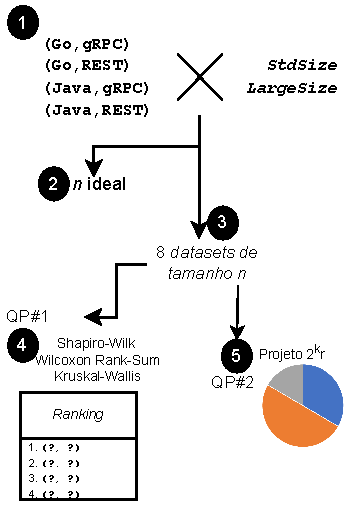
\includegraphics[width=0.6\linewidth]{imgs/metodologia.terra.pdf}
  % \vspace{-5pt}
  \caption{Metodologia}
  \label{fig:metodologia}
\end{figure}


\subsection{Ambiente}
O ambiente experimental foi configurado de forma a promover o menor erro experimental possível:\\[-0.2cm]

\noindent {\bf Hardware}. Intel Core i7 de 9ª geração e 16 GB de RAM.\\[-0.3cm]

\noindent {\bf Sistema operacional}. Ubuntu Server com instalação mínima, garantindo que nenhuma outra aplicação interferisse nos testes, 
proporcionando um ambiente controlado e consistente.\\[-0.3cm]

\noindent {\bf Software}. apenas Java 17 e Go 1.16. A escolha das versões foi motivada por sua estabilidade e suporte de longo prazo, garantindo um ambiente de desenvolvimento confiável.\\[-0.3cm]

\noindent {\bf Servidor de aplicação}. \okterrasblp{Para Java, utilizou-se o Tomcat 10.1.8 para a implementação REST e gRPC Netty 1.56.1 para gRPC.
%{\em framework} Spring Boot 3.1.0 que inclui o servidor Tomcat 10.1.8. 
Go, por outro lado, já possui funcionalidades embutidas para servir HTTP no pacote \mcode{net/http}, utilizado em ambas as implementações}.\\[-0.3cm]
%, tornando desnecessário um servidor de aplicação separado}.\\[-0.2cm]

\noindent {\bf Coleta}. Durante a coleta, a aplicação alvo, seja qual for a implementação, foi configurada para rodar com a máxima prioridade (\textit{nice level} de -20), enquanto a aplicação cliente foi configurada com um \textit{nice level} de -19.

\subsection{Aplicação Alvo}
\label{sec:target-app}

No âmbito desse experimento, tem-se quatro implementações distintas de uma mesma aplicação, cada uma representando uma combinação única de linguagem de programação e estilo arquitetural de comunicação: \gogrpc{}, \gorest{}, \javagrpc{} e \javarest{}.
O propósito central da aplicação é a implementação de um único \textit{endpoint}, o qual tem a função crítica de receber um conjunto de números e, a partir desse conjunto, selecionar e exibir três elementos em posições aleatórias.
Essa metodologia deliberadamente simplificada foi adotada com o objetivo de isolar e quantificar com precisão o impacto exercido tanto pela linguagem de programação quanto pelo estilo arquitetural de comunicação sobre o desempenho geral do sistema. Essa abordagem reduz significativamente a possibilidade de interferência por variáveis externas ao experimento.

Além disso, a operação selecionada para ser realizada pela aplicação foi cuidadosamente escolhida para assegurar que o \textit{payload} completo seja efetivamente transferido para o serviço em questão, prevenindo assim qualquer forma de otimização prematura na leitura e processamento dos dados.
Essa premissa é de vital importância para o estudo, uma vez que uma parcela substancial das discrepâncias observadas entre os diferentes estilos arquiteturais advém especificamente da maneira como os dados são encapsulados e transportados por meio da rede.
Em consequência, é imperativo avaliar com minúcia o impacto que a transformação desses dados, de sua forma bruta para um formato que seja manejável pela linguagem de programação, tem sobre o desempenho geral.

Uma aplicação
%\footnote{A aplicação foi desenvolvida em Go, porém trata-se de uma aplicação de coleta de dados, sendo sua linguagem de implementação indiferente para o experimento.} 
é responsável por orquestrar os testes e coletar dados de desempenho.
%
%e persisti-los em um banco de dados SQL (\textit{Structured Query Language}) para análise subsequente.
São feitas $n$ requisições para cada um dos seguintes tipos de \textit{payloads}:

O \textit{payload} \aspas{\textit{StdSize}} compreende um arranjo de 200 números inteiros com valores aleatórios entre 0 e 1.000, totalizando 0,763 KB.
Esse tamanho é representativo do tamanho médio de requisições HTTP comumente observadas em aplicações web, servindo como um \textit{benchmark} relevante para análises de desempenho \cite{chromium2012spdy}.
%
O \textit{payload} \aspas{\textit{LargeSize}} \space é concebido para ser exatamente 1.024 vezes maior que o \aspas{\textit{StdSize}}, refletindo uma carga significativamente mais pesada. Isso eleva o tamanho do \textit{payload} \aspas{\textit{LargeSize}} para 781,312 KB. 

Essa escala ampliada é crucial para testar o desempenho das implementações sob condições extremas de carga, permitindo uma investigação %detalhada 
sobre como diferentes tamanhos de \textit{payload} afetam o desempenho nas aplicações distribuídas.

\subsection{Coleta de Dados}
\label{sec:coletadados}

O procedimento experimental é delineado em $r=5$ repetições, cada uma contendo $n = 77$ requisições. 
%
Utilizou-se uma fórmula que permitiu definir o número de requisições ideal para a amostra com base em um conjunto de observações preliminares.
Considerando um nível de confiança de 95\% e 9 graus de liberdade (10 observações preliminares), a variável~\(z\) tem o valor de 1,833 e representa o valor crítico da distribuição t de \textit{Student} para esse nível de confiança e graus de liberdade especificados. O parâmetro \(r\) é definido como o erro tolerável, fixado em 5\%. A fórmula geral para o cálculo do tamanho da amostra (\(sz\)) 
%para cada combinação de linguagem de programação e estilo arquitetural 
é dada por \cite{jain1991}:
\begin{equation}
sz = \left( \frac{100 \cdot z \cdot s}{r \cdot \bar{x}} \right)^2
\end{equation}

onde:
\begin{itemize}
    \item \(s\) é o desvio padrão das medições prévias,
    \item \(\bar{x}\) é a média das medições prévias,
    \item \(z\) é o valor t de \textit{Student} para o nível de confiança e
    \item \(r\) é o erro percentual tolerável.
\end{itemize}

Durante cada repetição, a aplicação calcula o tempo despendido de cada requisição e as armazena em memória.
Esse processo é repetido até que todas as repetições previstas sejam concluídas.
Na fase final, 
esses dados são exportados para 
oito arquivos com $n$ tempos de execução,
um arquivo para cada uma das quatro implementações e
para cada um dos dois tamanhos de requisição,
e importados no R para análises estatísticas~\cite{R}.

\subsection{Análise de Desempenho ({\em QP\#1})}
Esta seção provê respostas à questão de pesquisa \#1 por meio da aplicação de procedimentos estatísticos em uma das cinco repetições dos dados coletados conforme descrito na Seção~\ref{sec:coletadados}. 


A Figura \ref{fig:smallBoxplot} ilustra um gráfico \textit{boxplot} comparando os
tempos de execução das quatro implementações \gogrpc{}, \gorest{}, \javagrpc{} e \javarest{} no cenário de requisições {\em StdSize}.
%
Cada caixa representa a distribuição dos tempos de resposta de diferentes configurações de aplicativos. A parte inferior da caixa indica o primeiro quartil (Q1), ou seja, 25\% dos dados são inferiores a esse valor, enquanto a parte superior mostra o terceiro quartil (Q3), com 75\% dos dados abaixo desse ponto. O espaço entre Q1 e Q3, conhecido como intervalo interquartílico (IQR), oferece uma medida da dispersão dos dados. A linha dentro da caixa marca a mediana, que é o valor central dos dados. Pontos individuais, ou \textit{outliers}, representam dados que se distanciam significativamente dos demais, geralmente definidos como valores que estão além de 1,5 vezes o IQR a partir dos quartis.


\begin{figure}[!ht]
    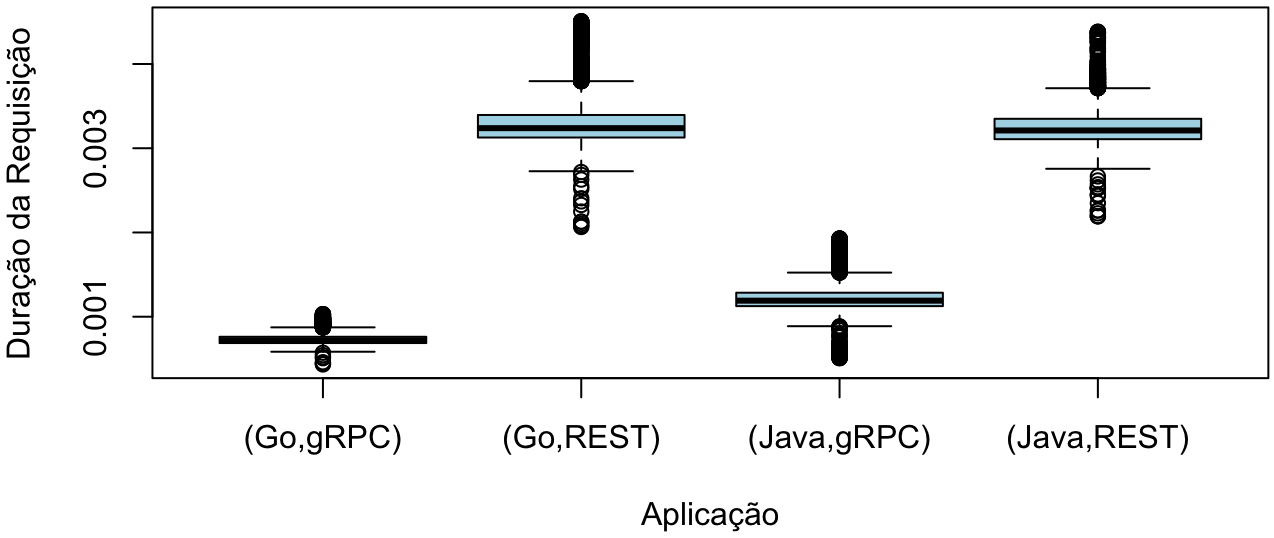
\includegraphics[width=.9\linewidth]{imgs/small.png}
    % \vspace{-10pt}
    \caption{Desempenho em requisições \textit{StdSize}}
    \label{fig:smallBoxplot}
\end{figure}

%valor das requisições para quatro combinações de linguagem de programação (Go e Java) e estilo arquitetural de comunicação (gRPC e REST) no cenário de requisições (\textit{LargeSize}). 

%para cada implementação \gogrpc{}, \gorest{}, \javagrpc{} e \javarest{} e tamanho de requisição {\em StdSize} e {\em LargeSize}.

No gráfico, é possível observar que combinações que utilizam gRPC têm desempenho melhor que as que utilizam REST, além de que a espessura das caixas indicam que existe uma variabilidade menor quando se utiliza a arquitetura de comunicação~gRPC.



A Figura \ref{fig:bigBoxplot}, de forma complementar, ilustra um gráfico {\em boxplot}
similar, porém no cenário de requisições {\em LargeSize}.
% comparando o valor das requisições para as mesmas quatro combinações de linguagem de programação e estilo arquitetural de comunicação no cenário de requisições (\textit{StdSize}). 
Nota-se no gráfico que aplicações que usam REST possuem desempenho superior as que usam gRPC.

\begin{figure}[!ht]
    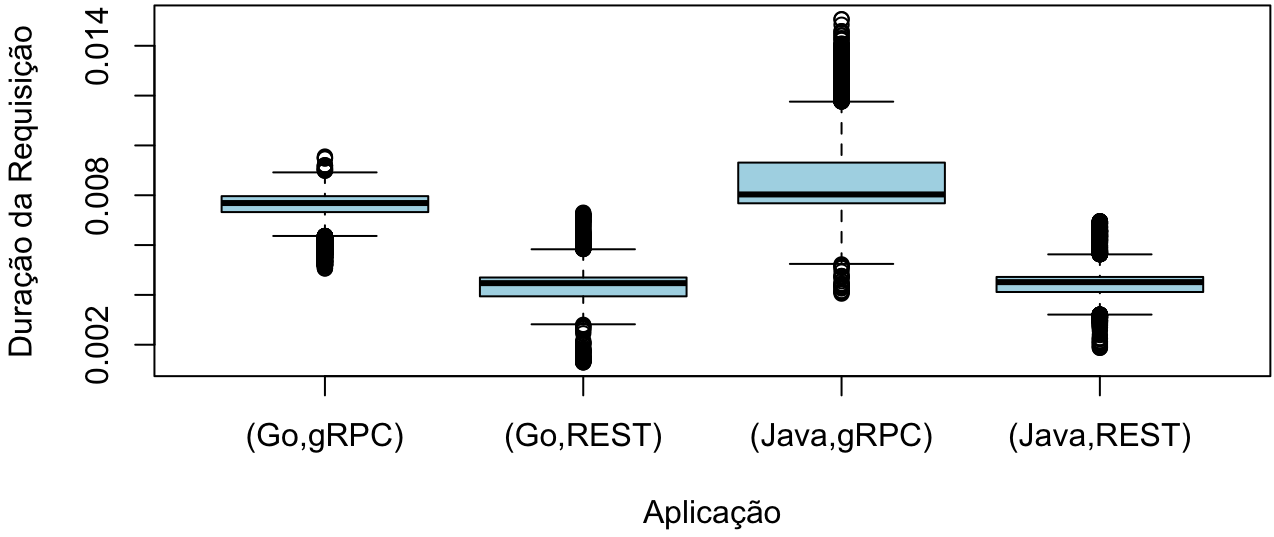
\includegraphics[width=.9\linewidth]{imgs/big.png}
    % \vspace{-10pt}
    \caption{Desempenho em requisições \textit{LargeSize}}
    \label{fig:bigBoxplot}
\end{figure}


A Tabela~\ref{tab:mediadesempenho} reporta os dados de mediana e desvio padrão. 
%
Nota-se diferenças significativas entre os cenários de requisições~\textit{StdSize} e \textit{LargeSize}. Por um lado, nas requisições~\textit{StdSize}, a implementação \gogrpc{} apresentou o menor tempo médio de resposta, destacando-se também por seu baixo desvio padrão, o que indica uma regularidade notável no desempenho. 
%
Por outro lado, nas requisições~\textit{LargeSize}, a implementação~\gorest{} apresentou o menor tempo médio, complementado por um desvio padrão relativamente baixo, sugerindo relativa estabilidade mesmo sob condições de cargas de grande volume.

\begin{table}[!ht]
\small
\centering
\caption{Mediana do desempenho com desvio padrão}
\label{tab:mediadesempenho}
\begin{tabular}{lrrrr}
%\hline
& \multicolumn{2}{c}{\textbf{\em StdSize}} & \multicolumn{2}{c}{\textbf{\em LargeSize}} \\
%\hline
\textit{Implementação} & \textit{Mediana} & \textit{Desvio} & \textit{Mediana} & \textit{Desvio} \\
%\hline
\gogrpc{} & 0,00071 & 0,00006 &  0,00768 & 0,00070\\
\gorest{} & 0,00323 & 0,00028 & 0,00447 & 0,00067\\
\javagrpc{} & 0,00119 & 0,00017 & 0,00803 & 0,00134\\
\javarest{} & 0,00321 & 0,00023 & 0,00451 & 0,00066

%\hline
% \rowcolor{gray!50} \multicolumn{3}{c}{\textbf{LargeSize}} \\
% %\hline
% \javarest{} & 0.00443 & 0.00066 \\
% \javagrpc{} & 0.00836 & 0.00134 \\
% \gorest{} & 0.00436 & 0.00067 \\
% \gogrpc{} & 0.00752 & 0.00070 \\
%\hline
\end{tabular}
\end{table}

\noindent{\bf Normalidade dos dados}. A análise de normalidade dos dados desempenhou um papel crucial antes de proceder com testes estatísticos. Para os tempos de execução de todas as oito combinações, 
o teste de Shapiro-Wilk indicou que os dados {\em não} seguiam uma distribuição normal.

Como esse teste possui uma sensibilidade grande para pequenos desvios de normalidade~\cite{miot_2017}
quando utilizado em grandes quantidades de amostras (como neste estudo), métodos visuais de análise como gráficos Q-Q e histogramas foram empregados para confirmar a suposição e avaliar a distribuição dos tempos de resposta das implementações. Essas análises confirmaram a não-normalidade dos dados, um achado significativo que orientou a escolha de técnicas estatísticas adequadas para a análise subsequente \cite{Habibzadeh2024}. A não-normalidade dos dados é uma característica comum em conjuntos de dados reais, especialmente em medições de desempenho de sistemas computacionais, onde fatores externos e a própria natureza das tecnologias podem influenciar grandemente a variação dos dados \cite{Holovnia2023}.

Dada essa característica dos dados, optou-se por métodos não paramétricos para as análises seguintes.
A escolha foi fundamentada pela capacidade desses métodos de fornecer resultados confiáveis sem a necessidade de pressupostos de normalidade, essenciais em testes paramétricos.
Essa decisão metodológica assegura que as comparações de desempenho entre as diferentes combinações de linguagens e estilos arquiteturais de comunicação sejam válidas e não comprometidas por violações das premissas estatísticas \cite{Holovnia2023}.
Portanto, a análise de normalidade não apenas informou a escolha dos testes estatísticos apropriados, mas também reforçou a robustez das inferências estatísticas realizadas nesse estudo \cite{Habibzadeh2024}.\\[-0.2cm]

\noindent{\bf Diferenças estatisticamente relevantes}. 
Conforme abordado na Seção~\ref{sec:metodosestatisticos}, 
o teste de Wilcoxon \textit{Rank-Sum} é um método não paramétrico utilizado para comparar duas amostras independentes. O método é ideal para dados que não seguem uma distribuição normal e é aplicado quando se deseja determinar se duas distribuições possuem a mesma mediana sem assumir a normalidade dos dados. Dada a sua capacidade de adaptar-se às condições do estudo, o teste de Wilcoxon pode ser implementado em suas formas condicionais, com classificações naturais e intermediárias, para analisar eficazmente as diferenças entre as medianas \cite{Pokropp1992}.

A Tabela~\ref{tab:wilcoxon} reporta os resultados dos testes de Wilcoxon, tanto para requisições~\textit{StdSize} quanto para \textit{LargeSize}. Os resultados indicaram diferenças estatisticamente significativas em todas as comparações 
entre as combinações.
%de linguagens de programação e estilos arquiteturais de comunicação.
{A comprovação de todos os pares serem estatisticamente diferentes permite comparar as medianas e classificar os melhores pares de tecnologias.}

% Por exemplo, as comparações entre Java com REST e Java com gRPC, bem como entre Java com REST e Go com gRPC, mostraram variações significativas de desempenho.
% Essas variações sugerem uma eficácia distinta do gRPC em melhorar o desempenho em relação ao REST, independentemente da linguagem usada.
% Além disso, a diferença entre Go com REST e Go com gRPC também destacou uma superioridade de desempenho do gRPC.
% Esses resultados são fundamentais para compreender quais configurações de linguagem e arquitetura de comunicação proporcionam melhor desempenho em aplicações distribuídas, influenciando decisões técnicas para a otimização de sistemas.

\begin{table}[!ht]
    \centering
    \small
    \caption{Wilcoxon {\em Rank Sum}: resultados $p$-valor }
    \vspace{-6pt}
    \begin{tabular}{lrr}
        %\hline
        \textbf{Comparação} & \textbf{\textit{StdSize}} & \textbf{\textit{LargeSize}} \\
        %\hline
        \javarest{} vs. \javagrpc{} & < 2,2e-16 & < 2,2e-16\\
        \javarest{} vs. \gorest{} & 4,532e-09 & < 2,2e-16\\
        \javarest{} vs. \gogrpc{} & < 2,2e-16 & < 2,2e-16\\
        \javagrpc{} vs. \gorest{} & < 2,2e-16 & < 2,2e-16\\
        \javagrpc{} vs. \gogrpc{} & < 2,2e-16 & < 2,2e-16\\
        \gorest{} vs. \gogrpc{} & < 2,2e-16 & < 2,2e-16\\
        %\hline
    \end{tabular}
    \label{tab:wilcoxon}
\end{table}

O teste de Kruskal-Wallis é especialmente útil para analisar variações em dados categóricos, como os avaliados nesse estudo, onde é analisado o impacto de diferentes linguagens de programação e estilos arquiteturais de comunicação no desempenho das aplicações.
%
{Esse teste foi empregado em conjunto com o teste de Wilcoxon \textit{Rank-Sum} para reforçar os resultados obtidos e garantir que as comparações entre as implementações sejam válidas.}

Tabela~\ref{tab:kruskal} reporta os resultados do teste de Kruskal-Wallis. Primeiramente, conforme esperado, o teste indicou que tanto o estilo arquitetural de comunicação quanto a linguagem de programação têm um impacto significativo no desempenho das aplicações, com diferenças estatisticamente relevantes observadas tanto em requisições \textit{StdSize} quanto \textit{LargeSize}.
Em segundo lugar, os resultados indicam que tanto a escolha do estilo arquitetural de comunicação quanto a linguagem de programação  afetam o desempenho.
Por último, mas não menos importante, quando as variáveis de estilo arquitetural de comunicação e linguagem de programação foram combinadas para análise, a interação entre esses dois fatores mostrou um efeito ainda mais pronunciado no desempenho.
%
Estudos como os realizados por Habibzadeh~\cite{Habibzadeh2024} ilustram a aplicabilidade do teste de Kruskal-Wallis em contextos diversos, reforçando a importância de considerar não apenas os efeitos isolados de cada variável, mas também como elas interagem entre si.\\[-0.3cm]


\begin{table}[!ht]
    \centering
    \small
    \caption{Kruskal-Wallis: resultados}
    \vspace{-8pt}
    \begin{tabular}{lrr}
        %\hline
        & \multicolumn{2}{c}{\textbf{\em StdSize / LargeSize}} \\
        \textit{Comparação} & \textit{Chi-quadrado} & \textit{$p$-valor} \\
        %\hline

        %\hline
        arq.~comunicação & 21,806 / 22,500 & < 2,2e-16~/~< 2,2e-16 \\
        linguagem & 1,239,3 / 356,88 & < 2,2e-16~/~< 2,2e-16 \\
        fator combinado & 24,624 / 22,988 & < 2,2e-16~/~< 2,2e-16 \\
        %\hline
        % \rowcolor{gray!50} \multicolumn{3}{c}{\textbf{\em LargeSize}} \\
        % %\hline
        % estilo arq. de comunicação & 22.500 & < 2.2e-16 \\
        % linguagem & 356,88 & < 2.2e-16 \\
        % fator combinado & 22.988 & < 2.2e-16 \\
        % \hline
    \end{tabular}
    \label{tab:kruskal}
\end{table}

\noindent{\bf\em Ranking}. Considerando que há uma diferença estatisticamente significativa entre as medianas, é possível classificar o desempenho dos pares.
A Tabela~\ref{tab:rankings} exibe a lista das implementações ordenadas da melhor para a pior, considerando as requisições~\textit{StdSize} e \textit{LargeSize}. Essa ordenação identifica quais combinações de linguagem e arquitetura de comunicação oferecem o melhor desempenho, auxiliando na escolha das tecnologias mais eficientes para aplicações distribuídas.

\begin{table}[!ht]
    \centering
    \small
    \caption{{\em Rankings} das implementações}
    \vspace{-8pt}
    \begin{tabular}{crr}
        %\hline
        \textbf{Posição} & \multicolumn{1}{c}{\textbf{\textit{StdSize}}} & \multicolumn{1}{c}{\textbf{\textit{LargeSize}}} \\
        %\hline
        \#1 & \gogrpc{}, 0,00071s & \gorest{}, 0,00447s \\
        \#2 & \javagrpc{}, 0,00119s & \javarest{}, 0,00451s \\
        \#3 & \javarest{}, 0,00321s & \gogrpc{}, 0,00768s \\
        \#4 & \gorest{}, 0,00323s &\javagrpc{}, 0,00803s \\
        %\hline
    \end{tabular}
    \label{tab:rankings}
\end{table}

Nesses resultados, observa-se uma influência significativa do tamanho da requisição, \textit{StdSize} ou \textit{LargeSize}, e da combinação entre linguagem e estilo arquitetural de comunicação sobre o desempenho das implementações. Os resultados indicam que 
\textit{\gogrpc{}} mostrou superioridade em requisições {\em StdSize}, enquanto \gorest{} e \javarest{} se destacaram -- quase de forma equivalente -- nas requisições {\em LargeSize}. 
Essa distinção é particularmente relevante no projeto de sistemas distribuídos, onde a escolha do estilo arquitetural de comunicação pode afetar significativamente a eficiência operacional. 
Por um lado, a arquitetura de comunicação gRPC, com sua forma de comunicação mais leve e baseado em RPC, provou ser mais eficiente em requisições usuais, possivelmente devido à
eficiência na compactação de dados e na redução da latência e da sobrecarga de comunicação.
Por outro lado, a arquitetura de comunicação REST mostrou-se mais adaptada para requisições de grande volume, provavelmente devido 
à flexibilidade do REST em lidar com grandes volumes de dados sem estrutura rígida. 

\subsection{Influência dos Fatores ({\em QP\#2})}
Esta seção provê respostas à questão de pesquisa \#2 por meio da condução de um projeto estatístico nas cinco repetições dos dados coletados conforme descrito na Seção~\ref{sec:coletadados}. 


Para entender o impacto de cada fator no desempenho das aplicações distribuídas, utilizou-se o projeto fatorial \(2^{k}r\) com 2 fatores e 5 repetições. 
Esse projeto experimental permite a análise sistemática dos efeitos principais e das interações entre os fatores~\cite{jain1991}.
O projeto \(2^{k}r\) é uma extensão do projeto fatorial \(2^{k}\), incluindo repetições para estimar o erro experimental e aumentar a precisão dos resultados.

Os fatores escolhidos para o experimento foram a linguagem de programação e o estilo arquitetural de comunicação. A linguagem de programação (A) variou entre Go (-1) e Java (+1), enquanto o estilo arquitetural de comunicação (B) variou entre gRPC (-1) e REST (+1). Esses fatores são fundamentais para aplicações distribuídas modernas, onde a escolha da tecnologia pode impactar significativamente o desempenho.

Tabela~\ref{tab:sinais} reporta, respectivamente, as tabelas de sinais utilizadas para o projeto fatorial \(2^{2}r\) para requisições \textit{StdSize} e \textit{LargeSize} incluindo os totais por fator e os totais divididos por 4, também conhecido como efeito do fator. Foram combinadas as duas tabelas de sinais pois apenas as duas última linhas se diferem. Por exemplo, pode-se dizer que o 
efeito do fator linguagem de programação para requisições {\em StdSize} foi de 0,00017
e para requisições {\em LargeSize} foi de 0,00019.

\begin{table}[!ht]
    \small
    \centering
    \caption{Projeto Fatorial \(2^{2}r\) - \textit{StdSize}}
    \vspace{-5pt}
    \begin{tabular}{ccccc}
        %\hline
        \textbf{I} & \textbf{\small Ling.} & \textbf{\parbox{1.4cm}{\centering \small Arq. com.}} & \textbf{\small Interação} & {\small \textbf{Impl.}} \\
        %\hline
        1 & -1 & -1 & 1 & \gogrpc{} \\
        1 & 1 & -1 & -1 & \javagrpc{} \\
        1 & -1 & 1 & -1 & \gorest{} \\
        1 & 1 & 1 & 1 & \javarest{} \\
        %\hline
        0,00973 & 0,00070 & 0,00526 & -0,00082 & $Total_{Std}$\\
        0,00243 & 0,00017 & 0,00131 & -0,00020 & $Total_{Std}/4$ \\
        &\\[-0.3cm]
        %\hline
        0,02486 & 0,00079 & -0,00599 & -0,00049 & $Total_{Large}$\\
        0,00621 & 0,00019 & -0,00149 & -0,00012 & $Total_{Large}/4$ \\
        %\hline
    \end{tabular}
    \label{tab:sinais}
\end{table}

Com os efeitos de cada fator, são calculadas as seguintes sete somas de quadrados para obter de fato as influências de cada fator:
(i)~SSY~\textit{(Soma dos Quadrados Total dos Dados)} que representa a totalidade da variação observada nos dados, somando os quadrados de cada valor de resposta coletado; 
(ii)~SSE~\textit{(Erro da Soma dos Quadrados)} que corresponde à variação em \(Y\) que não é explicada pelos fatores no modelo e é calculada subtraindo a contribuição dos fatores e suas interações do SSY;
(iii)~SS0~\textit{(Soma dos Quadrados do Total)} que é a soma associada ao efeito total, que engloba todos os efeitos sistemáticos observados;
(iv)~SST~\textit{(Soma dos Quadrados dos Tratamentos)} é a variação que é explicada apenas pelos tratamentos, calculada subtraindo SS0 de SSY; 
(v)~SSL~\textit{(Soma dos Quadrados da Linguagem)} que quantifica o quanto da variação total em \(Y\) é explicada pelas diferenças entre as linguagens de programação utilizadas;
(vi)~SSAC~\textit{(Soma dos Quadrados da Arquitetura de Comunicação)} que avalia o impacto do estilo arquitetural de comunicação sobre a variação nos dados; e
(vii)~SSLAC~\textit{(Soma dos Quadrados da Interação Linguagem e Arquitetura de Comunicação)} que mede a interação entre os fatores Linguagem e Arquitetura de Comunicação, indicando se o efeito de uma variável sobre o desempenho depende da outra.


Dado que $E_T$ é o Efeito Total, 
$E_L$ é o Efeito Linguagem de Programação,
$E_{AC}$ é o Efeito Arquitetura de Comunicação,
e $E_I$: Efeito Interação,
as Equações 2 a 8 transcrevem as fórmulas para cada soma de quadrados incluindo os valores resultantes
no formato $v_{StdSize}/v_{LargeSize}$, onde $v_{StdSize}$ é o resultado para o projeto
fatorial de requisições {\em StdSize} e $v_{LargeSize}$ de requisições {\em LargeSize}.

\vspace{-5pt}
\begin{footnotesize}
\begin{eqnarray}
\label{eq:projeto}
SSY &= \sum (Y_{ij}^2)&{= 0,00015/0,00081} \\
SSE &= SSY - 2^{k}r \left( E_T^2 + E_L^2 + E_{AC}^2 + E_I^2 \right) &{= 8,84833/5,74272} \\
SS0 &= 2^{k}r E_T^2 &{= 0,00011/0,00077} \\
SST &= SSY - SS0 &{= 3,70512/4,65600} \\
SSL &= 2^{k}r E_L^2 &{= 6,20191/7,90081} \\
SSAC &= 2^{k}r E_{AC}^2 &{= 3,47041/4,48847} \\
SSLAC &= 2^{k}r E_I^2 &{= 8,42123/3,10969}
\end{eqnarray}
\end{footnotesize}

Por fim, as influências de cada fator no resultado final são calculadas como porcentagens das somas de quadrados sobre a soma total dos quadrados. A Tabela~\ref{tab:influencia} reporta, portanto, as influências dos fatores para as requisições \textit{StdSize} e \textit{LargeSize}.

\begin{table}[!ht]
    \small
    \centering
    \caption{Influência dos Fatores no Desempenho}
    \label{tab:influencia}
    \vspace{-5pt}
    \begin{tabular}{ccc}
        %\hline
        \textbf{Fator} & \textbf{\textit{StdSize}} & \textbf{\textit{LargeSize}} \\
        %\hline
        Linguagem de programação & 1,67\% & 1,69\% \\
        Arquitetura de comunicação & 93,66\% & 96,40\% \\
        Interação & 2,27\% & 0,66\% \\
        Erro & 2,38\% & 1,23\% \\
        %\hline
    \end{tabular}
\end{table}

A aplicação do projeto fatorial \(2^{k}r\) mostrou que o estilo arquitetural de comunicação é o principal fator que influencia o desempenho de aplicações distribuídas, sendo responsável por aproximadamente 94\% do impacto em requisições de tamanho padrão ({\em StdSize}) e superando 96\% em requisições de grande volume ({\em LargeSize}).

A influência da linguagem de programação, embora presente, é menos pronunciada comparativamente ao estilo arquitetural de comunicação. 
Esses resultados enfatizam a importância de selecionar o estilo arquitetural de comunicação adequado para otimizar o desempenho de sistemas distribuídos, oferecendo um suporte claro para decisões técnicas no desenvolvimento de software distribuído.

A influência da interação foi até superior à influência da linguagem de programação para requisições {\em StdSize}, porém 
praticamente nula (0,66\%) para requisições {\em LargeSize}, o que indica que a interação é contextual e dependente do tamanho da requisição, sendo mais relevante em cenários com cargas menores e menos impactante em situações com volumes de dados maiores.

Por fim, a influência do erro é relativamente pequena, indicando que o modelo experimental utilizado é robusto e confiável.

\subsection{Ameaças à validade}
Pelo menos três ameaças à validade podem ser mencionadas:\\[-0.3cm]

\noindent{\em Hardware e software}. Otimizações das linguagens de programação, de processadores, uso de memória e interferência dos serviços do Ubuntu podem ter afetado as mensurações de tempo. No entanto, pode-se alegar que todas as decisões de projeto do experimento foram tomadas antes de qualquer mensuração e afeta as linguagens de programação e os estilos arquiteturais de comunicação da mesma forma.\\[-0.3cm]

\noindent{\em Tamanho das requisições}.  Embora os tamanhos \textit{StdSize} e \textit{LargeSize} tenham sido projetados para representar, respectivamente, cargas médias e substancialmente maiores que a média, a definição de \aspas{média} pode não capturar adequadamente a variabilidade dos tamanhos de requisição encontrados em aplicações do mundo real. Trabalhos futuros na linha de uso de mais métricas são propostos para ajudar a refletir a distribuição real de tamanhos de requisição em aplicações distribuídas, onde requisições podem variar significativamente em tamanho e frequência.\\[-0.3cm]

\noindent{\em Aplicação}. \okterrasblp{No escopo deste estudo, a aplicação alvo foi projetada propositalmente para isolar -- ao máximo -- o experimento de fatores externos. De forma complementar, experimentos com aplicações que demandem aspectos particulares das linguagens de programação, como concorrência e paralelismo, são vislumbrados como trabalhos futuros.}\\[-0.3cm]

Essas ameaças destacam a necessidade de cautela ao interpretar os resultados e ao considerar a aplicabilidade das conclusões para outros contextos ou configurações. É essencial reconhecer que, enquanto os resultados fornecem {\em insights} valiosos sobre o desempenho relativo das tecnologias estudadas sob condições específicas, a generalização desses resultados para outros cenários deve ser feita com uma compreensão clara das limitações e contextos em que os testes foram realizados.

\subsection{Replicabilidade}
Os aplicativos utilizados e os dados coletados durante o estudo estão publicamente disponíveis em: 
\begin{center}
\vspace{-7pt}
{\fbox{\url{https://github.com/PqES/2024_sblp}}}
\end{center}


\section{Trabalhos Relacionados}
\label{sec:tr}
Esta seção descreve trabalhos relacionados ao estudo empírico conduzido neste artigo.

Śliwa e Pańczyk~\cite{restGraphqlGrpc} avaliam o desempenho das arquiteturas de comunicação REST, GraphQL e gRPC, destacando-se o REST pela quantidade de transações por segundo e o gRPC pela eficiência na transmissão de dados. O estudo proporciona um pano de fundo relevante para a presente pesquisa, que também examina o desempenho de diferentes arquiteturas de comunicação, mas se preocupa com o fator das linguagens Java e Go, além de utilizar métodos estatísticos robustos para avaliar o impacto dessas arquiteturas em diversos tamanhos de requisição. Contrariamente, a pesquisa inclui a análise de GraphQL e não emprega análises estatísticas avançadas como o teste de Wilcoxon \textit{Rank-Sum} ou Kruskal-Wallis utilizados neste trabalho. Portanto, enquanto ambos os estudos contribuem para a compreensão do desempenho de diferentes tecnologias de comunicação, o presente trabalho distingue-se pela sua abordagem metodológica e foco analítico específico.

Bora e Bezboruah~\cite{restSoap} publicaram dois serviços web distintos, um utilizando a arquitetura SOAP e outro com arquitetura REST, ambos implementados em Java. Eles realizaram uma avaliação comparativa desses serviços, empregando o {\em Mercury Load Runner} para testes de carga e estresse. A análise estatística dos resultados revelou que a arquitetura REST mostrou-se mais eficiente e escalável em comparação com SOAP. Esse resultado é semelhante ao encontrado no presente trabalho, onde a arquitetura REST também mostrou maior eficiência em requisições de grande volume, embora o presente estudo usa uma abordagem estatística mais rigorosa com testes específicos para medir diferenças de desempenho.

Abhinav et al.~\cite{javaVsGo} analisa a concorrência entre Go e Java por meio de experimentos com algoritmos de multiplicação de matrizes e {\em PageRank}. Os autores identificam que Go apresenta melhor desempenho em menor número de cálculos, enquanto Java supera à medida que o volume de cálculos aumenta. Esse padrão se inverte quando considerado a criação e gerenciamento de {\em threads}, com Java mostrando vantagem em computações menores e Go melhorando em cenários mais exigentes. Ambas as linguagens possuem características únicas de concorrência, destacando-se em diferentes aplicações.
{No contexto do presente trabalho, não existem cálculos numerosos sendo realizados nas implementações alvo, isso pode explicar a baixa influência da linguagem de programação nos resultados. }

Marx et al.~\cite{htt1Vshttp2} analisam as características de desempenho do HTTP/2 em comparação ao HTTP/1.1. \noterrasblp{, destacando o impacto das inovações tecnológicas como a multiplexação de múltiplos recursos em uma única conexão TCP, estratégias avançadas de priorização, {\em Server Push} e compressão de cabeçalho HPACK} 
Os experimentos revelam que, apesar das melhorias propostas, o HTTP/2 apresenta limitações significativas em condições de rede adversas, onde a conexão multiplexada pode se tornar um gargalo e os benefícios em termos de desempenho raramente superam os do HTTP/1.1, exceto na redução de sobrecarga. {É relevante mencionar que a arquitetura de comunicação gRPC, utiliza o HTTP/2 como base, o que influencia diretamente o seu desempenho em comparação ao REST, que tradicionalmente utiliza o HTTP/1.1.}

Kamiński et al.~\cite{kaminski2023comparative} conduzem uma análise comparativa das arquiteturas de comunicação de Internet mais usados, incluindo REST, \textit{WebSocket}, gRPC, GraphQL e SOAP. Utilizando servidores web implementados em Python, a equipe mediu o tempo e a sobrecarga de transferência de dados em operações específicas. Concluiu-se que o gRPC foi o método mais eficiente e confiável, enquanto o GraphQL mostrou-se o mais lento e problemático em termos de uso em servidores web.
{Esse estudo utilizou cargas pequenas para os comparativos e seus resultados em relação às arquiteturas de comunicação corroboram com os obtidos no presente trabalho com cargas semelhantes.}

Berg e Redi~\cite{berg2023benchmarking} conduziram um estudo comparativo sobre o desempenho de \textit{throughput} de requisições entre chamadas de API convencionais baseadas em REST e gRPC.
O estudo foi realizado com uma metodologia bem definida, desenvolvida pelos próprios autores, sem o uso de métodos estatísticos tradicionais.
Os servidores %REST e gRPC 
foram implementados em três linguagens de programação (Java, Python e Rust) e os testes de \textit{benchmark} foram conduzidos em uma rede local para avaliar o desempenho de requisições em diferentes tamanhos de carga.
Os resultados indicaram que, embora o REST inicie com um desempenho melhor para cargas menores, o gRPC supera o REST à medida que o tamanho da carga útil aumenta, oferecendo um \textit{throughput} superior em mensagens de maior tamanho. Embora possa parecer que o resultado é o oposto do encontrado neste estudo, os estudos se complementam e apresentam comportamentos opostos em diferentes métricas ({\em throughtput} vs.~tempo de execução).

\section{Conclusão}
\label{sec:conclusao}
A motivação para este estudo surgiu da necessidade crescente de desenvolver APIs robustas e eficientes que possam atender às exigentes demandas de desempenho e escalabilidade de sistemas de software atuais. Diante disso, 
foi conduzido um estudo empírico que emprega procedimentos estatísticos rigorosos para quantificar as melhorias oferecidas por uma linguagem de programação e um estilo arquitetural de comunicação considerados promissores dentro de um contexto de sistemas distribuídos, abordando especificamente Go e Java e gRPC e REST. 

A pesquisa foi impulsionada por duas principais questões de pesquisa: (i)~qual a combinação mais eficiente entre as linguagens de programação Go e Java e os estilos arquiteturais de comunicação gRPC e REST e (ii)~qual a influência da linguagem de programação e do estilo arquitetural de comunicação na eficiência. 

A questão de pesquisa~\#1 evidenciou que Go apresenta desempenho superior tanto em requisições \textit{StdSize} quanto \textit{LargeSize}, 
comparado ao Java. Esse resultado sugere que a seleção de Go em combinação com gRPC, pode oferecer vantagens substanciais em termos de eficiência, especialmente em ambientes que requerem comunicações frequentes e de alto desempenho.

A questão de pesquisa~\#2 conclui que -- de fato -- a influência da arquitetura de comunicação é de 94\% no desempenho.
\okterrasblp{
Isso indica que, ao substituir REST por gRPC, existem cenários em que fábricas de software podem ter uma melhoria de desempenho em seus sistemas 
sem necessitar de uma reescrita de código em uma linguagem de programação diferente.}

A diferença de desempenho entre REST e gRPC nos diferentes tamanhos de requisição pode ser atribuída a diversos fatores inerentes às duas arquiteturas de comunicação. O gRPC, por ser baseado no protocolo HTTP/2 e utilizar a serialização Protobuf, é mais eficiente em termos de latência e consumo de recursos para transmissões de dados menores devido à sua capacidade de multiplexação de múltiplas chamadas em uma única conexão. Já o REST, com sua simplicidade e ampla adoção, tende a ser mais eficiente para requisições maiores, possivelmente devido à sua capacidade de lidar com cargas de dados mais pesadas e menos dependência de conexões simultâneas.

Trabalhos futuros incluem: 
(i)~avaliar a eficiência com requisições de diversos tamanhos a fim de encontrar pontos de transição onde uma arquitetura de comunicação pode superar outra; 
(ii)~avaliar a eficiência com diferentes frequências de solicitações, a fim de obter os limiares de desempenho de REST e gRPC em situações de estresse;
(iii)~avaliar em diferentes configurações de infraestrutura como rede, CPU, memória, etc.; e
\okterrasblp{(iv)~avaliar o desempenho com algoritmos específicos no servidor, a fim de medir o impacto de funcionalidades especificas das linguagens, como paralelismo e gerenciamento de memória.}

\chapter{CONCLUSÃO}
\label{cap:conclusao}

A motivação para este estudo surgiu da necessidade crescente de desenvolver APIs robustas e eficientes que possam atender às exigentes demandas de desempenho e escalabilidade de sistemas de software atuais. Diante disso, 
foi conduzido um estudo empírico que emprega procedimentos estatísticos rigorosos para quantificar as melhorias oferecidas por uma linguagem de programação e um estilo arquitetural de comunicação considerados promissores dentro de um contexto de sistemas distribuídos, abordando especificamente Go e Java e gRPC e REST. 

A pesquisa foi impulsionada por duas principais questões de pesquisa: (i)~qual a combinação mais eficiente entre as linguagens de programação Go e Java e os estilos arquiteturais de comunicação gRPC e REST e (ii)~qual a influência da linguagem de programação e do estilo arquitetural de comunicação na eficiência. 

A questão de pesquisa~\#1 evidenciou que Go apresenta desempenho superior tanto em requisições \textit{StdSize} quanto \textit{LargeSize}, 
comparado ao Java. Esse resultado sugere que a seleção de Go em combinação com gRPC, pode oferecer vantagens substanciais em termos de eficiência, especialmente em ambientes que requerem comunicações frequentes e de alto desempenho.

A questão de pesquisa~\#2 conclui que -- de fato -- a influência da arquitetura de comunicação é de 94\% no desempenho.
\okterrasblp{
Isso indica que, ao substituir REST por gRPC, existem cenários em que fábricas de software podem ter uma melhoria de desempenho em seus sistemas 
sem necessitar de uma reescrita de código em uma linguagem de programação diferente.}

\noterrasblp{A diferença de desempenho entre REST e gRPC nos diferentes tamanhos de requisição pode ser atribuída a diversos fatores inerentes às duas arquiteturas de comunicação. O gRPC, por ser baseado no protocolo HTTP/2 e utilizar a serialização Protobuf, é mais eficiente em termos de latência e consumo de recursos para transmissões de dados menores devido à sua capacidade de multiplexação de múltiplas chamadas em uma única conexão. Já o REST, com sua simplicidade e ampla adoção, tende a ser mais eficiente para requisições maiores, possivelmente devido à sua capacidade de lidar com cargas de dados mais pesadas e menos dependência de conexões simultâneas.}

Trabalhos futuros incluem: 
(i)~avaliar a eficiência com requisições de diversos tamanhos a fim de encontrar pontos de transição onde uma arquitetura de comunicação pode superar outra; 
(ii)~avaliar a eficiência com diferentes frequências de solicitações, a fim de obter os limiares de desempenho de REST e gRPC em situações de estresse;
(iii)~avaliar em diferentes configurações de infraestrutura como rede, CPU, memória, etc.; e
\okterrasblp{(iv)~avaliar o desempenho com algoritmos específicos no servidor, a fim de medir o impacto de funcionalidades especificas das linguagens, como paralelismo e gerenciamento de memória.}


%==============================================================================
% Incluindo bibliografia
%\bibliographystyle{plain}             % estilo para labels em numeros
%\bibliographystyle{alpha}             % estilo para labels em iniciais
\bibliographystyle{abntex2-alf}           % estilo para referências usando ABNT, 
                                       % precisa instalar o abntex para usar!!!

%inclui Referências Bibliográficas
%inclui Referências Bibliográficas
\referencias
\bibliography{refbib}			% arquivo exemplo refbib.bib
%==============================================================================
% Incluindo anexos num1erados com letras maiusculas.
%\apendices
% \apendice{O que são apêndices}
\label{cap:apendice}

Um apêndice é um suporte elucidativo e ilustrativo do texto principal. Sua função é agrupar elementos que são úteis à compreensão do texto e que, no entanto, podem ser apresentados à parte sem prejuízo à compreensão. É útil para a apresentação de modelagens, diagramas extensos, listagens de código-fonte de programas e demais elementos que o autor julgar necessário à complementação do tema abordado no texto principal.


%==============================================================================
% Fim do texto
\end{document}
